\documentclass[conference]{IEEEtran}

\usepackage[utf8]{inputenc}
\usepackage{cite}
\usepackage{amsmath,amssymb,amsfonts}
\usepackage{graphicx}
\graphicspath{{figures/}{../figures/}}
\usepackage{booktabs}
\usepackage{multirow}
\usepackage{array}
\usepackage{url}
\usepackage{xurl}
\usepackage{hyperref}
\usepackage{xcolor}
\usepackage{enumitem}
\usepackage{float}
\usepackage{placeins}
\usepackage{stfloats}

\setlength{\dbltextfloatsep}{8pt plus 1pt minus 2pt}

\hypersetup{
    colorlinks=true,
    linkcolor=black,
    citecolor=black,
    urlcolor=blue,
    hypertexnames=false
}

\title{When Online Attention Spills Over: Consumer Goods, Platform Control, and Government Response in China}

\author{
\IEEEauthorblockN{Hanyu Xie}
\IEEEauthorblockA{
Columbia University \\
 hx2413@columbia.edu
}
\and
\IEEEauthorblockN{Haotian Lei}
\IEEEauthorblockA{
Columbia University \\
 hl3945@columbia.edu
}
}

\begin{document}

\maketitle

\begin{abstract}
In order to examines how social media originated controversies in China move beyond platform in term of specific discussion and become associated with offline spillovers in consumer goods, markets, and government response. Rather than treating ``online trends'' as a broad or self-evident category, we will focuses on high visibility controversies that begin or intensify in Chinese social media environment and then become visible across a wider public attention space, including news coverage, search behavior, investor attention, consumer behavior, and official response.

We developed a threshold--pathway--spillover framework. The claim is that online controversies in China do not become consequential simply because they are popular on social media. They become consequential when they break through a governed visibility environment and become legible to consumers, markets, or state actors. The first three cases focus on consumer goods spillovers: the 2024 Nongfu Spring controversy as a brand-boycott and reputation damage pathway, the 2023 Japan wastewater salt panic as a panic-buying and supply reassurance pathway, and the late 2022 Lianhua Qingwen episode as a demand of medicine and pharmaceutical-repricing pathway. The fourth case which is the Urumqi fire and Zero COVID reversal is treated separately as a boundary case, aim to show how politically sensitive attention can also break through platform control and become associated with government response.

Because high-quality historical data from Weibo, Douyin or WeChat, and Xiaohongshu are difficult to obtain, this paper does not claim to directly measure domestic Chinese social media visibility. Google Trends is used only as a secondary proxy for broader cross platform public salience after a controversy has already moved beyond the original platform environment. The analysis put together Google Trends with event timelines, media reports, market data, policy actions, and survey evidence from 104 respondents with experience in Chinese social media and some familiarity with U.S. or Western social media. The paper does not make strong causal claims, instead, it identifies patterned associations between visibility breakthroughs and offline spillovers under conditions of partial platform data.
\end{abstract}

\section{Introduction}
\subsection{Background}
The controversies in social media do not always remain inside. In many cases, a dispute that begins as scattered online discussion becomes visible across platforms, news coverage, investor attention, consumer behavior, and official response. Where we aim to studies that process in China, where platform visibility is shaped not only solely by user activity, but also by recommendation systems, trending lists, moderation practices, search filtering, and state regulation. The central issue is therefore not simply whether a topic appears online. The critical question is that when an online controversy becomes visible enough to matter outside the platform.

This distinction is especially important in the Chinese context. Public controversies may circulates through Weibo, Douyin, WeChat, Xiaohongshu, short video re-posting, screenshots, private group chats, and news coverage at the same time. Yet these channels are not equally observable to us. A historical platform data with high quality from Chinese social media platforms are difficult to collect consistently, especially after an event has passed. For example, the case Urumqi Fired is under censorship. For that reason, this research does not attempt to reconstruct the full domestic platform ecology of each controversy. What we trying to do is to study how selected controversies moved from platform specific discussion into broader public salience and whether that broader visibility was temporally associated with consumer goods or government spillovers.

By doing such, it also avoids a common measurement problem. Google Trends cannot be used as a direct substitute for Weibo, Douyin, WeChat, or Xiaohongshu data, especially because Google is not normally accessible to ordinary users in mainland China and Google Trends measures normalized search interest rather than social-media discussion volume \cite{googlechina2010,googlechina2012,googletrendsfaq}. In this paper, Google Trends will be used more narrowly: as a secondary indicator of externalized, cross platform attention after a China related controversy has become visible beyond its original domestic social media environment. The data in Google Trends are interpreted alongside media reports, market indicators, policy timelines, and survey responses, not as a stand-alone measure of Chinese public opinion.

\subsection{Research Question}
\emph{In China, how do social media originated controversies move beyond platform specific discussion into broader public attention, and how are these visibility breakthroughs associated with consumer goods spillovers and government response?}

We focuses mainly on consumer goods and market spillovers. The first three cases examine how online visibility is associated with brand damage, panic buying, and product-linked demand. A fourth case, which is the Urumqi fire and Zero COVID reversal, will be a boundary case. Because this case is not a relevant to consumer goods. It is included because it shows how politically sensitive attention can also exceed platform control and become associated with policy response.

\subsection{Argument}
What we argue is that in China online controversies do not influences offline behavior because they are trending on social media. They become consequential because when they break through platform level visibility or censorship controls and spread into broader public attention. Once that visibility threshold is crossed, then such event will be form of spillover depends on the type of event. Brand controversies may produce reputation damage and market decline. The fears in public health may produce panic buying and supply reassurance. Medicine related attention may produce demand expectations and stock repricing. Last but not least, politically sensitive crises may generate policy pressure and government response.

The contribution of this paper is not simply a claim that social media directly causes every observed market or policy outcome. The more cautious claim is that visibility breakthroughs are temporally associated with different forms of offline spillover. The analysis identifies these associations through a structured comparison of cases, not through a full causal model.

\subsection{Contributions}

The study makes four contributions. First, the study narrows the object of analysis. Instead of treating ``online trends'' as a broad category, we focus on social media originated controversies that will move beyond platform specific discussion, then becomes visible in a wider public attention environment. By such it separates ordinary online discussion from high visibility events that are more likely to generate observable spillovers.

Second, the study clarify measurement role of Google Trends. Google Trends is not use as a direct measure of domestic Chinese social media activity. In contrast, Google Trends is treated as a secondary indicator of broader cross platform salience after an event that is already moved beyond its original platform. The use of Google Trend measure is interpreted together with market data, event timelines, policy actions, media reports, and survey responses.

Third, what this study distinguishes among different spillover pathways is that not treating offline impact as a single outcome. The Nongfu Spring case illustrates a brand boycott and reputation damage pathway; the salt panic case illustrates a panic buying and supply reassurance pathway; and the Lianhua Qingwen case illustrates a medicine demand and pharmaceutical repricing pathway. The Urumqi fire is included separately as a boundary case, showing how politically sensitive visibility can become associated with government response rather than consumer goods behavior.

Lastly, the study adds survey. The survey is not nationally representative and is not used as causal evidence. Its purpose is more niche: it helps assess whether the selected events were recognizable among respondents with Chinese social media experience and whether respondents perceived algorithms, trending lists, and government response as shaping event visibility. They survey will strengthens the study by use of partial platform data without overstating what the survey can prove.

\section{Related Literature}

\subsection{Platform Governance and Visibility Control in China}

The study is builds on recent scholarship that treats platform visibility as a governed process rather than a purely organic outcome of user discussion. Online visibility is shaped by recommendation systems, hot-search lists, search filtering, content moderation, platform responsibility, and state regulation in China. The 2022 Internet Information Service Algorithmic Recommendation Management Provisions are especially relevant because they each covers personalized recommendation, ranking and selection, search filtering, dispatching and decision-making, and there are also other algorithmic technologies used to distribute information to users \cite{digichina2022algorithmic}. The provisions also restrict the manipulation of topic lists, hot-search terms, search-result rankings, and other forms of information presentation that could influence online public opinion \cite{digichina2022algorithmic}. This supports our claim that attention in China does not circulate in a neutral information market. It moves through a visibility environment where amplification and restriction are both governed.

There is also a recent scholarship on China's algorithmic regulation makes this point more explicit. Yang and Yao argue that the social media in China's algorithmic recommendation rules extend state oversight into the recommendation systems used by major online platforms, making algorithmic distribution a formal regulatory object rather than a purely technical design choice \cite{yang2022algorithmic}. Xu and Yu's work on internet and digital media governance in the Xi Jinping era provides a broader institutional background, emphasizing the centrality of state authority, platform responsibility, and regulatory control in China's digital media system \cite{xu2022regulating}. Chin, Park, and Li's comparative study of false-information governance in Chinese and American social media platforms also helps clarify that platform governance differs across institutional settings, especially in the balance between state regulation, platform self-regulation, and co-regulation \cite{chin2022falseinfo}. Together, these studies support the theoretical basis for ours governed-visibility framework: online controversies in China may spread quickly, but their spread is mediated by platform infrastructures and regulatory constraints.

These researches also help clarify the meaning of platform control in this study. Platform control does not mean that all sensitive information disappears, also does not mean that all viral attention is artificially manufactured. Rather, control refers to a set of institutional and technical mechanisms that would shape whether a topic becomes visible, how long it remains visible, and which public can easily encounter it. Even though algorithms and trending lists may amplify a topic, meanwhile moderation and search filtering may restrict or redirect it. This is a dual process that is central to the study's threshold argument: an online controversy becomes consequential when it breaks through this controlled visibility environment and becomes legible to consumers, markets, or government.

\subsection{Online Firestorms and Thresholds of Public Attention}

The research on online firestorms provides the closest conceptual foundation for ours threshold logic. Kim et al.'s comparative study of Weibo and Twitter shows that online firestorms differ across national and platform contexts, including differences in targets, expressive styles, and the forms of public reaction that become visible \cite{kim2021firestorms}. Kim's findings are important for this study because they suggest that an online controversy's visibility is not solely determined by user anger. Those visibilities are also shaped by platform environment, topic category, and broader political and media conditions.

This study widen the insight by asking what happens after a controversy crosses certain visibility threshold. Much of the online-firestorm literature focuses on the online episode itself: how public criticism forms, spreads, and intensifies. The present studies instead follows the controversy beyond the platform and asks whether high visibility attention becomes associated with offline spillovers in consumer behavior, market response, or government action. In conclusion, our study does not treat virtuality as the endpoint of analysis. It treats visibility breakthrough as an intermediate stage between platform discussion and offline consequence.

In Chinese context, the threshold concept is very useful because online criticism could exist without becoming broadly visible or politically consequential. Many controversies may circulate inside a platform, within screenshots, or among private networks without creating measurable spillover. In contrast, a controversy that moves across social media, news coverage, search behavior, investor attention, and official response becomes more legible as a public event. That's the reason why ours threshold--pathway--spillover framework is designed to capture that difference.

\subsection{Consumer Nationalism, Brand Boycotts, and Consumer Video Activism}

In this paper, the consumer-goods cases also draw on recent work about consumer nationalism and digital consumer activism in China. Liao and Xia's study of the anti-Lotte boycott shows how Chinese internet users used digital media to coordinate a nationalist consumer boycott and connect purchasing behavior with national identity \cite{liao2023consumer}. Their analysis is directly relevant to the Nongfu Spring case because it shows that brand controversies in China may become more than ordinary consumer disputes. They can become public performances of identity, loyalty, and national belonging.

Research on consumer video activism further supports this paper's claim that consumer controversies can move from individual dissatisfaction to broader public visibility. Yu's empirical study of consumer video activism shows how Chinese consumers use short-video platforms to protest against businesses, attract attention, and seek responses from media or government departments \cite{yu2021video}. Yu and Xu's later work on the emergence of a Chinese consumer sphere similarly argues that short-video-based social media platforms have become tools for consumers to protect their rights and make commercial grievances publicly visible \cite{yu2023consumer}. These studies help explain why consumer-goods controversies can spill beyond ordinary purchasing choices. When a brand dispute becomes visible through social media, it may generate reputational pressure, consumer avoidance, or market reassessment.

This research support our interpretation of the Nongfu Spring controversy as a brand boycott and reputational-damage pathway. The case is not treated as proof that online attention alone caused the firm's stock movement. Instead, it is interpreted as a case where social media originated criticism, brand identity, media attention, and investor attention became temporally aligned. The consumer nationalism and consumer activism literature makes this pathway plausible by showing that Chinese digital consumers can use online visibility to pressure firms and attach broader social meanings to consumption.

\subsection{Online Attention, Panic Buying, and Market Response}

Another recent literature links online attention to consumer behavior and market response. Studies of Chinese financial markets show that stock returns, trading volume, and commodity market reactions could be assiciated with social media sentiment, investor attention, and media sentiment. Liu et al. examine China's commodity futures market and find that social-network sentiment predicts commodity futures returns, while investor attention has a significant positive relationship with returns and absolute returns \cite{liu2023commodity}. This supports ours treatment of the salt panic as a case where online fear and market attention moved together around a consumer goods shock.

There are also other studies provide broader support for the market spillover mechanism. Wang et al. find that social media sentiment can affect same-day stock returns by use experimental evidence from an online message forum, although the effect is short-lived \cite{wang2022sentiment}. Duan, Liu, and Wang study COVID-19 sentiment in China using official news media and Sina Weibo data, finding that COVID-related sentiment indices predicted Chinese stock returns and turnover rates during the early pandemic period \cite{duan2021covid}. These studies do not prove causality in ours cases, but they support the more cautious claim that online attention and sentiment can become market relevant information.

Research on panic buying and public-health fear is also relevant to the salt panic and Lianhua Qingwen cases. Li et al.'s study of Chinese public panic buying at the beginning of the COVID-19 outbreak shows that perceived risk, social-media use, and connection with close others contributed to panic-buying behavior \cite{li2022panic}. Hou et al.'s social-media surveillance preprint uses Sina Weibo, Baidu search, and Ali e-commerce marketplace data to track public attention, risk perception, emotional response, protective behavior, and panic buying during the COVID-19 outbreak \cite{hou2020public}. Because Hou et al. is a preprint, this paper uses it only as a methodological example rather than as core peer-reviewed evidence. Its value is to show what an ideal China based data design might look like: combining native social-media data, domestic search data, and e-commerce indicators. Because such historical platform data are not consistently available for all cases in this project, the present paper instead uses Google Trends, event timelines, market data, policy actions, and survey responses as combined evidence.

Together, these studies support our interpretation of the salt panic and Lianhua Qingwen cases. In the salt panic, online fear became associated with panic buying, salt-stock volatility, and government supply reassurance. In the Lianhua Qingwen case, reopening COVID era health uncertainty became associated with product specific attention, medicine demand expectations, pharmaceutical repricing, and later correction. The literature suggests that these patterns are plausible forms of online to offline spillover.

\subsection{Government Response and the Boundary Policy Case}

The reason why Urumqi fire is treated as a boundary case is because its main spillover not consumer purchasing behavior but government response. Recent work on protest and information control in China helps explain why politically sensitive visibility matters even in a controlled platform environment. Zheng and Meng's work on responsiveness and social protest in China shows that state response to public pressure is selective and institutionally shaped, rather than automatic \cite{zheng2021responsiveness}. This supports the paper's cautious interpretation of the Urumqi case: the event did not single-handedly cause the Zero COVID reversal, but it became part of a broader pressure environment in which public visibility was politically significant.

Information control research also clarifies the restrictive side of the platform environment. Ruan, Knockel, and Crete-Nishihata show that Chinese information control operates not only through censorship but also through public punishment and signaling repression, especially when online expression challenges government credibility or authority \cite{ruan2021punishment}. This helps explain why the Urumqi case should be treated separately from the consumer-goods cases. Its pathway involves politically sensitive attention, collective visibility, and state response, not ordinary market demand.

This literature supports the boundary case logic. The Urumqi case does not show that online attention directly caused policy reversal. Instead, it shows that even in a highly controlled platform environment, some politically sensitive controversies may become visible enough to enter the government's response environment. This strengthens the paper's broader claim that platform control does not eliminate online spillover. It changes the threshold and pathway through which spillover occurs.

\section{Case Selection}
The reason we select these four cases because we want these serve as sample of recent China related controversies in the post pandemic period. These cases were selected because each case satisfies four conditions: first, a clear triggering event. Second, visible discussion on or around Chinese socialmedia platforms. Third, observable spillover into consumer behavior, market indicators, or government response, and last enough public information to reconstruct a basic event timeline.

The first three were selected to serve core consumer goods comparison. What the Nongfu Spring controversy captures is a brand boycott and reputational damage pathway. Meanwhile, Japan wastewater salt panic captures a panic-buying pathway in which online fear became associated with consumer hoarding, salt-stock volatility, and government supply reassurance. Lastly, Lianhua Qingwen episode captures a medicine demand pathway in which reopening COVID era health concerns became associated with product specific attention and pharmaceutical-stock repricing.

The Urumqi fire will be included as a boundary case. Because Urumqi fire main spillover was not consumer purchasing behavior, but policy pressure and government response. It is analytically useful because it shows the outer limit of the paper's argument: when an online controversy becomes politically sensitive and highly visible, platform control may shape its visibility, but it may not fully prevent public pressure from becoming legible to the state.

\begin{table*}[t]
\centering
\caption{Case Selection Logic}
\label{tab:case_selection}
{\footnotesize
\setlength{\tabcolsep}{4pt}
\begin{tabular}{p{0.15\textwidth}p{0.17\textwidth}p{0.17\textwidth}p{0.17\textwidth}p{0.20\textwidth}}
\toprule
Case & Trigger & Main pathway & Primary spillover & Why included \\
\midrule
Nongfu Spring & Zong Qinghou's death and brand controversy & Brand boycott & Reputational damage and stock decline & Consumer-goods brand spillover \\
Salt panic & Japan wastewater release & Panic buying & Hoarding, salt-stock volatility, reassurance & Fast commodity panic \\
Lianhua Qingwen & Zero COVID relaxation and medicine concern & Medicine demand & Product attention and Yiling repricing & Product-linked demand shock \\
Urumqi fire & Residential fire and protest visibility & Boundary policy pathway & Government response and reopening repricing & Politically sensitive boundary case \\
\bottomrule
\end{tabular}
}
\end{table*}

\section{Measurement Strategy and Google Trends Limitation}
One of the core measurement challenges of the project is the limited high-quality historical data of China's social media platforms. Ideally, the analysis will use the archived Weibo hot search data, TikTok trend data, WeChat article circulation, Xiaohongshu participation and audit records. In practice, it is difficult to obtain this data consistently in each case, especially after the incident has passed. This restriction shapes the empirical strategy of the thesis.

For this reason, this article does not claim that Google Trends directly measures the attention of social media in China. This is especially important, because ordinary users in mainland China usually do not have access to Google. Google trends measure normalized search interest, not social media discussion volume\cite{googlechina2010,googlechina2012,googletrendsfaq}.
Therefore, it is misleading to regard Google Trends as a direct substitute for Weibo, TikTok, WeChat or Xiaohongshu.

On the contrary, Google Trends is used as a broader cross-platform public prominent secondary agent. Logic is that when the dispute based on China becomes large enough, it may go beyond its original domestic platform environment and appear in overseas Chinese discussions, Chinese and English news reports, investor search behavior, general public search interests and interpersonal discussions. Google Trends helps to identify these externalized attention peaks, but it cannot reveal the entire number, emotions, audit structures or algorithmic paths of social media discussions in China.

Therefore, this article triangularly analyzes Google trends with other evidence: event schedules, media reports, stock price and trading volume data, official statements, policy actions and survey results. In this design, Google Trend is not the main proof of Chinese opinion. This is an imperfect but comparable signal of whether the controversy has entered a broader public concern.

Unless otherwise stated, the case number combines Google trend search interest data with Investing.com historical price and trading volume data. The event window is reconstructed from the cited media and official sources. Survey visualization is based on the author survey output file in \texttt{survey\_outputs/} \cite{googletrendsfaq,investinghistorical}.

\begin{table}[t]
\centering
\caption{Google Trends Variables}
\label{tab:trends_variables}
\footnotesize
\begin{tabular}{p{0.34\columnwidth}p{0.56\columnwidth}}
\toprule
Case & Google Trends variables \\
\midrule
Nongfu Spring & ``Nongfu Spring,'' ``Wahaha'' \\
Salt panic & ``Japan nuclear wastewater,'' ``salt panic'' \\
Lianhua Qingwen & ``Lianhua Qingwen,'' ``Yiling Pharmaceutical,'' ``China COVID medicine'' \\
Urumqi fire & ``China protests,'' ``zero covid,'' ``Urumqi fire'' \\
\bottomrule
\end{tabular}
\end{table}
\FloatBarrier

\section{Survey-Based Triangulation of Event Awareness and Perceived Platform Control}
In order to reduce dependence on Google Trends, this article adds the survey evidence of 104 respondents. The sample is not representative of the whole country. It is best understood as a convenient sample of students, young professionals, Chinese immigrants and international students who have experience in using Chinese social media and have some familiarity with American or Western social media. This sample is very useful for studying perceived cross-platform awareness, but it cannot estimate China's national public opinion.

The survey supported the paper's decision to regard selected cases as identifiable high-visibility events. Most of the respondents had heard of these four incidents before participating in the survey. The approval rate of the Urumqi fire, the salt panic related to Japanese wastewater discharge, the Nongfu spring controversy and the Lianhua Qingwen debate are more than 60 percent. This is very important, because the case in the thesis is not an obscure example of choice after the fact. Among the respondents with relevant media experience, they are widely recognized.

Table~\ref{tab:survey_summary} summarizes the key survey findings. Appendix Fig.~\ref{fig:appendix_survey} reports the cleaned survey visualizations.

\begin{table}[t]
\centering
\caption{Key Survey Findings}
\label{tab:survey_summary}
\footnotesize
\begin{tabular}{p{0.58\columnwidth}p{0.32\columnwidth}}
\toprule
Survey item & Main result \\
\midrule
Heard of Urumqi fire & 71.2\% \\
Heard of Nongfu Spring controversy & 67.3\% \\
Heard of salt panic & 63.5\% \\
Heard of Lianhua Qingwen debate & 63.5\% \\
First learned through Chinese social media & 38.5\% \\
Agree algorithms/trending lists increased visibility & 60.6\% rated 4--5 \\
Agree moderation/censorship reduced visibility & 61.6\% rated 4--5 \\
Agree government likely responds to large online trend & 85.6\% rated 4--5 \\
\bottomrule
\end{tabular}
\end{table}

The survey also supports the cross-platform framework of the paper. A large part of the respondents first learned about these events through Chinese social media platforms such as Weibo, TikTok, WeChat or Xiaohongshu. Others first contact them through traditional news media, Western social media or friends, family and classmates. This pattern shows that these events are not limited to one platform. They have experienced a mixed concentration environment of interaction between social media, news, interpersonal networks and search behavior.

The results further show that the respondents believe that platform control both magnifies and limits visibility. Many respondents agreed that the platform algorithm or trend list improved the visibility of these events. At the same time, many people agree that auditing, censorship or platform intervention reduces visibility. This is very important for the argument of the thesis, because China's platform control should not be understood as just suppression or just amplification. Visibility is generated through two mechanisms. Some themes are promoted, some are restricted, and some themes become consequences, precisely because they have broken through this controlled environment.

The survey also links online visibility with perceived offline effects. Most respondents believe that online trends can bring about real changes in sales, shortages or brand reputation. Many respondents also reported that online discussions affected their own spending behavior, including finding more information before purchasing, delaying or avoiding purchases, changing brands or products, or purchasing additional products. These responses do not prove that online trends lead to market fluctuations observed in the case study, but they support the rationality of the consumer spillover mechanism.

Finally, the investigation supports the logic of the boundary case. Most respondents believe that when the online trend becomes big enough in China, the government may respond publicly. Many have also identified possible responses, such as official clarification, regulatory or administrative action, market intervention, or supply assurance. This does not prove that the government's actions were caused by online attention, but it helps explain why the Urumqi fire and salt panic are related to the framework of platform control and offline response.

Overall, the survey is used as a perception-based triangulation. It will not replace the platform data, nor will it establish a causal relationship. Its value lies in showing that the selected cases are identifiable, that respondents connect them with Chinese social media and cross-platform visibility, and that respondents believe that consumer and government spillover is a reasonable result of large-scale online trends.

\FloatBarrier

\section{Results}
\subsection{Results Overview}
Case analysis from consumer goods spillage to border policy cases. The first three cases examined the different ways in which the attention caused by social media is associated with consumer behavior and market response. The fourth case examines a politically sensitive event in which visibility is related to the government's reaction rather than consumer goods behavior.

The comparison revolves around three questions. First of all, what caused the online controversy? Second, how did the controversy shift from a platform-specific discussion to a wider public attention? Third, what type of spillover effect follows: brand damage, panic buying, product demand re-standardization or government response?

\subsection{Case 1: Nongfu Spring and Brand-Boycott Spillover}
The Nongfu Spring case represents the way of brand boycott. The trigger is not a formal regulatory event or a public health emergency, but a reputation dispute that developed after the death of Qinghou Zong, the founder of Wahaha, in February 2024. The online sympathy for Wahaha is related to the criticism of Nongfu Spring, and the discussion has developed into a broader boycott narrative around brand logo, nationalism and consumer loyalty \cite{caixin2024nongfu}. Figure~\ref{fig:nongfu_trends_stock} links the attention breakthrough with the beginning of the stock market decline.

\begin{figure}[t]
    \centering
    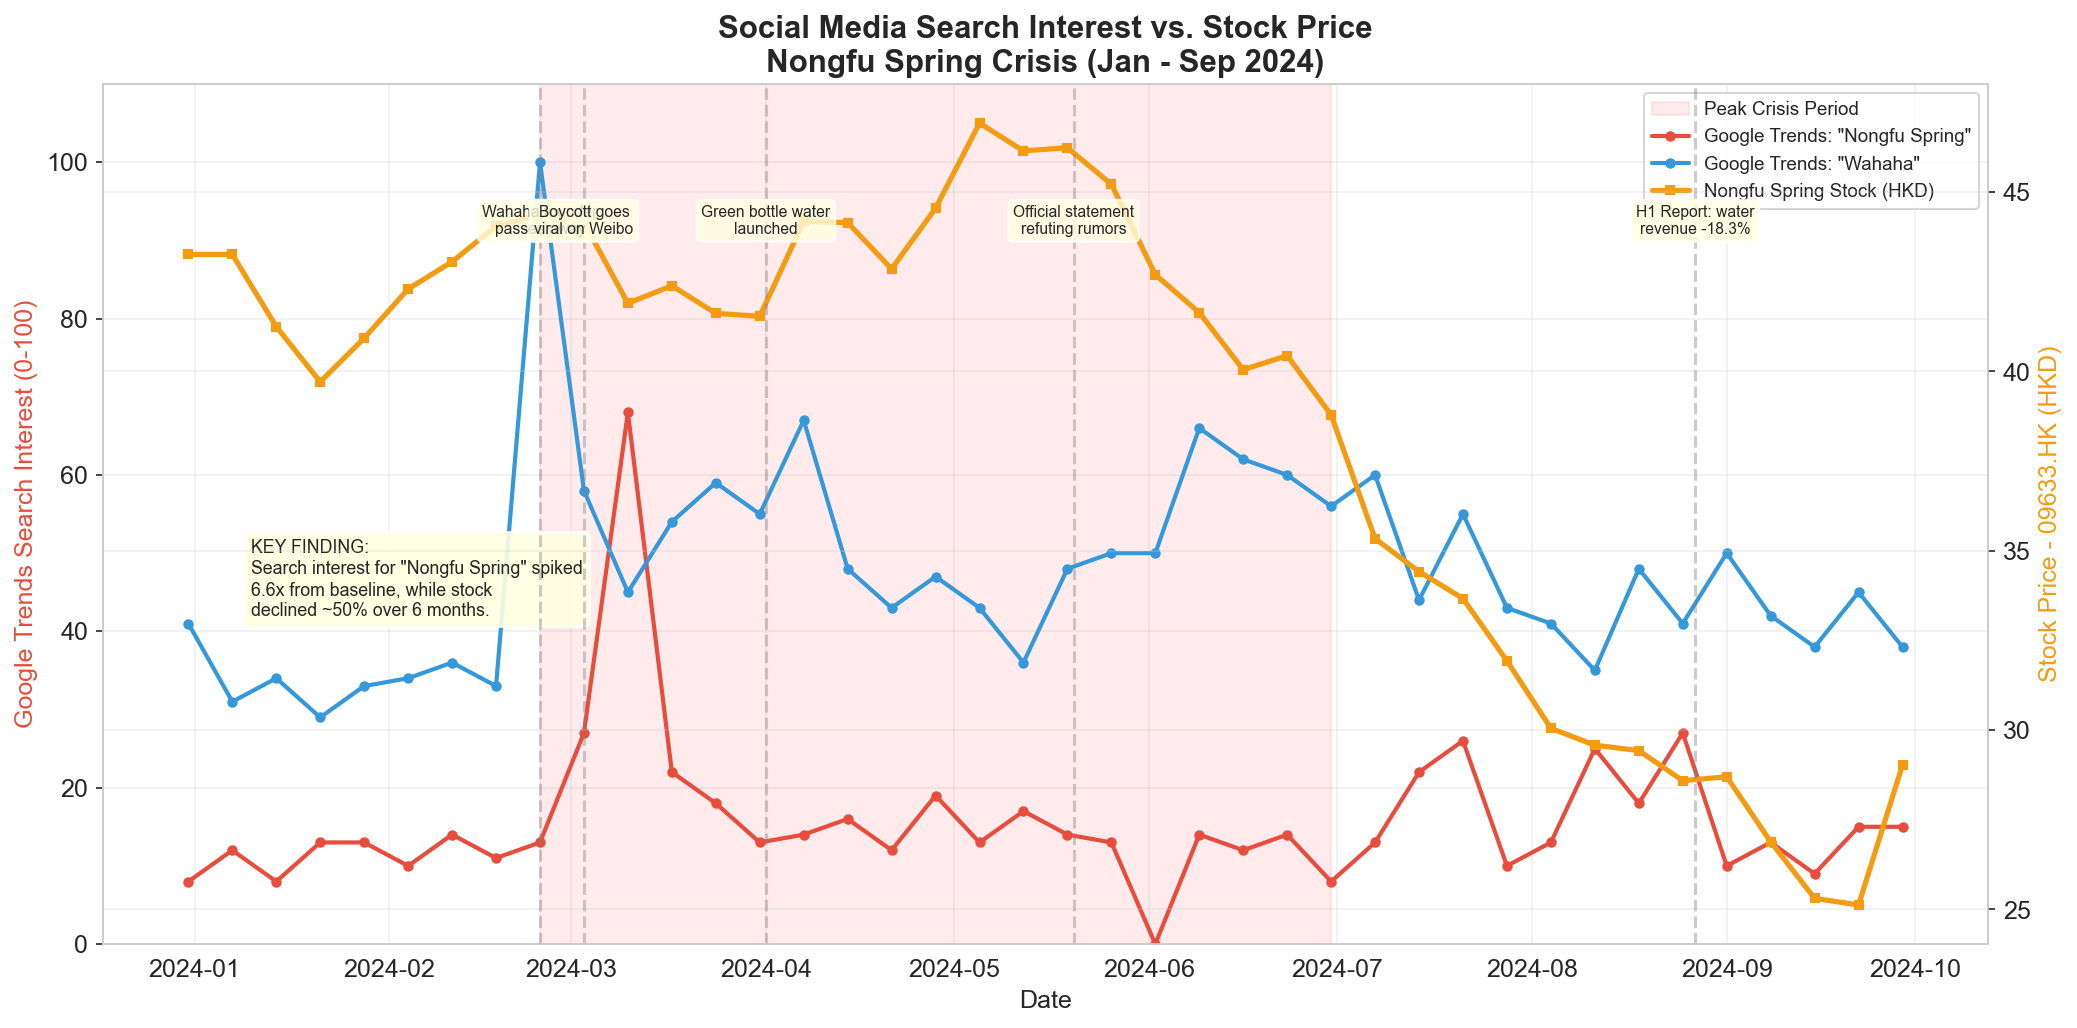
\includegraphics[width=\linewidth]{figures/Fig1_NongfuSpring_Trends_vs_Stock.png}
    \caption{Case 1: weekly search attention and Nongfu Spring stock price. The figure highlights the early-March visibility break and helps distinguish threshold crossing from the longer-run persistence that follows.}
    \label{fig:nongfu_trends_stock}
\end{figure}

The key point of this case is that the dispute is not just an online discussion. When the brand controversy enters a wider public position, it becomes more consequences. As shown in Figure~\ref{fig:nongfu_trends_stock}, search interests, media discussions, investor attention and stock market trends are temporarily consistent. In this sense, the case is in line with the broader arguments of this article: it becomes more important when the controversy breaks out from the discussion on a specific platform and becomes clear to consumers and investors. Figure~\ref{fig:nongfu_price_volume} then shows that the price drop and heavier transactions continue to exceed the initial trigger window.

\begin{figure}[t]
    \centering
    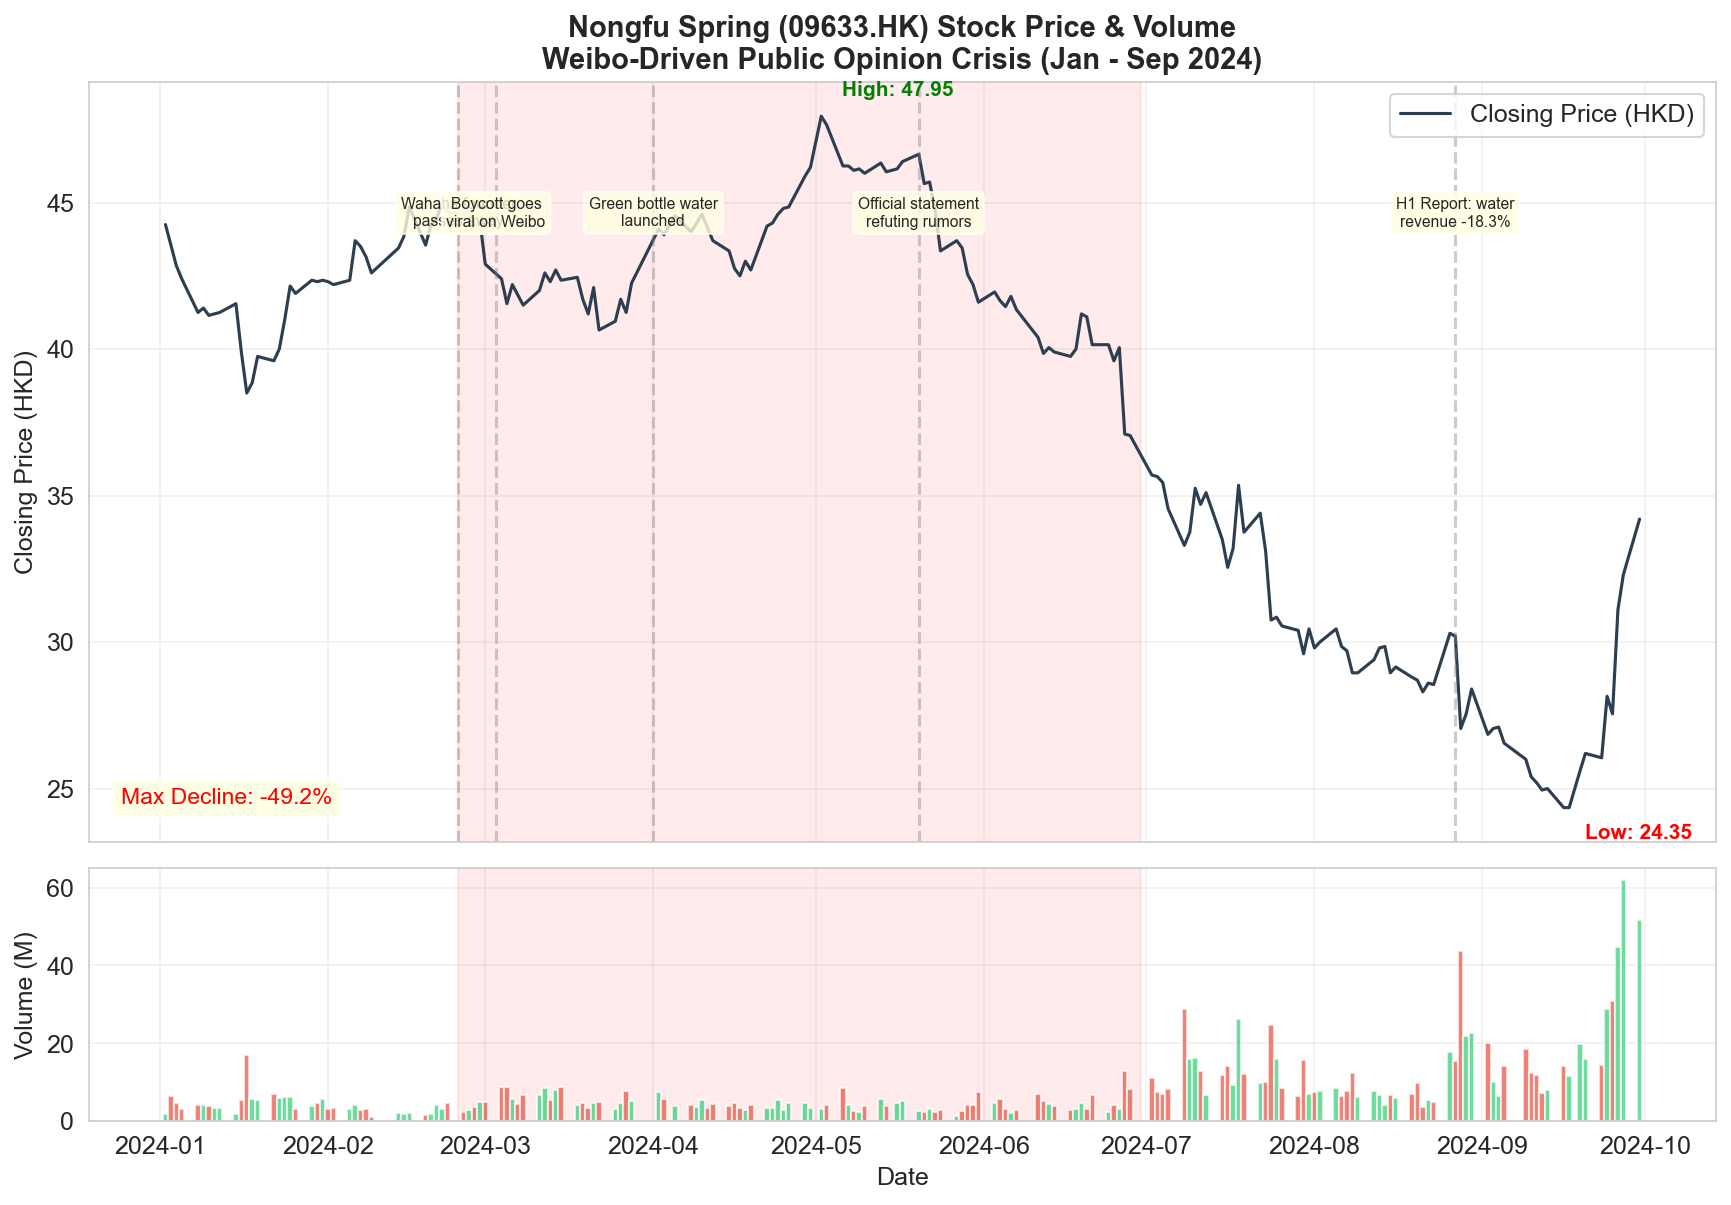
\includegraphics[width=\linewidth]{figures/Fig2_NongfuSpring_Price_Volume.png}
    \caption{Case 1: Nongfu Spring price and volume. The persistent decline and elevated trading activity distinguish slow-burn reputational damage from a short correction cycle.}
    \label{fig:nongfu_price_volume}
\end{figure}

The main spillover effect is continuous reputation and market damage, rather than a brief panic surge. The decline in stocks is not limited to the initial outburst of attention, which indicates that the controversy has been incorporated into a long-term reassessment of brand value and consumer sentiment. This makes Nongfuquan different from the salt panic case, in which the attention of the salt panic case soars and the market response is sharper, but shorter.

The case does not prove that online attention alone causes the stock to fall. Other commercial, market and financial factors may also play a role. However, timing supports the explanation related to online visibility and reputation overflow. Among the three consumer goods cases, Nongfu Spring showed the slowest but most lasting path.

\subsection{Case 2: Japan Wastewater Salt Panic and Panic-Buying Spillover}
The salt panic case represents the way of panic buying and supply assurance. The event was that in august 2023 the nuclear wastewater which discharged from Japan, which raised public worries about food safety and salt. Online discussions help turn geopolitical and public health issues into consumer goods panic. The result is not only talked by people, but also hoarding behavior, stock fluctuations in the salt industry and official supply guarantee\cite{reuters2023saltpanic,reuters2023saltmaker,li2022panic}.  Figure~\ref{fig:salt_trends_stocks} shows how attention surges and the salt fan stock response are concentrated in the same short window.

\begin{figure}[t]
    \centering
    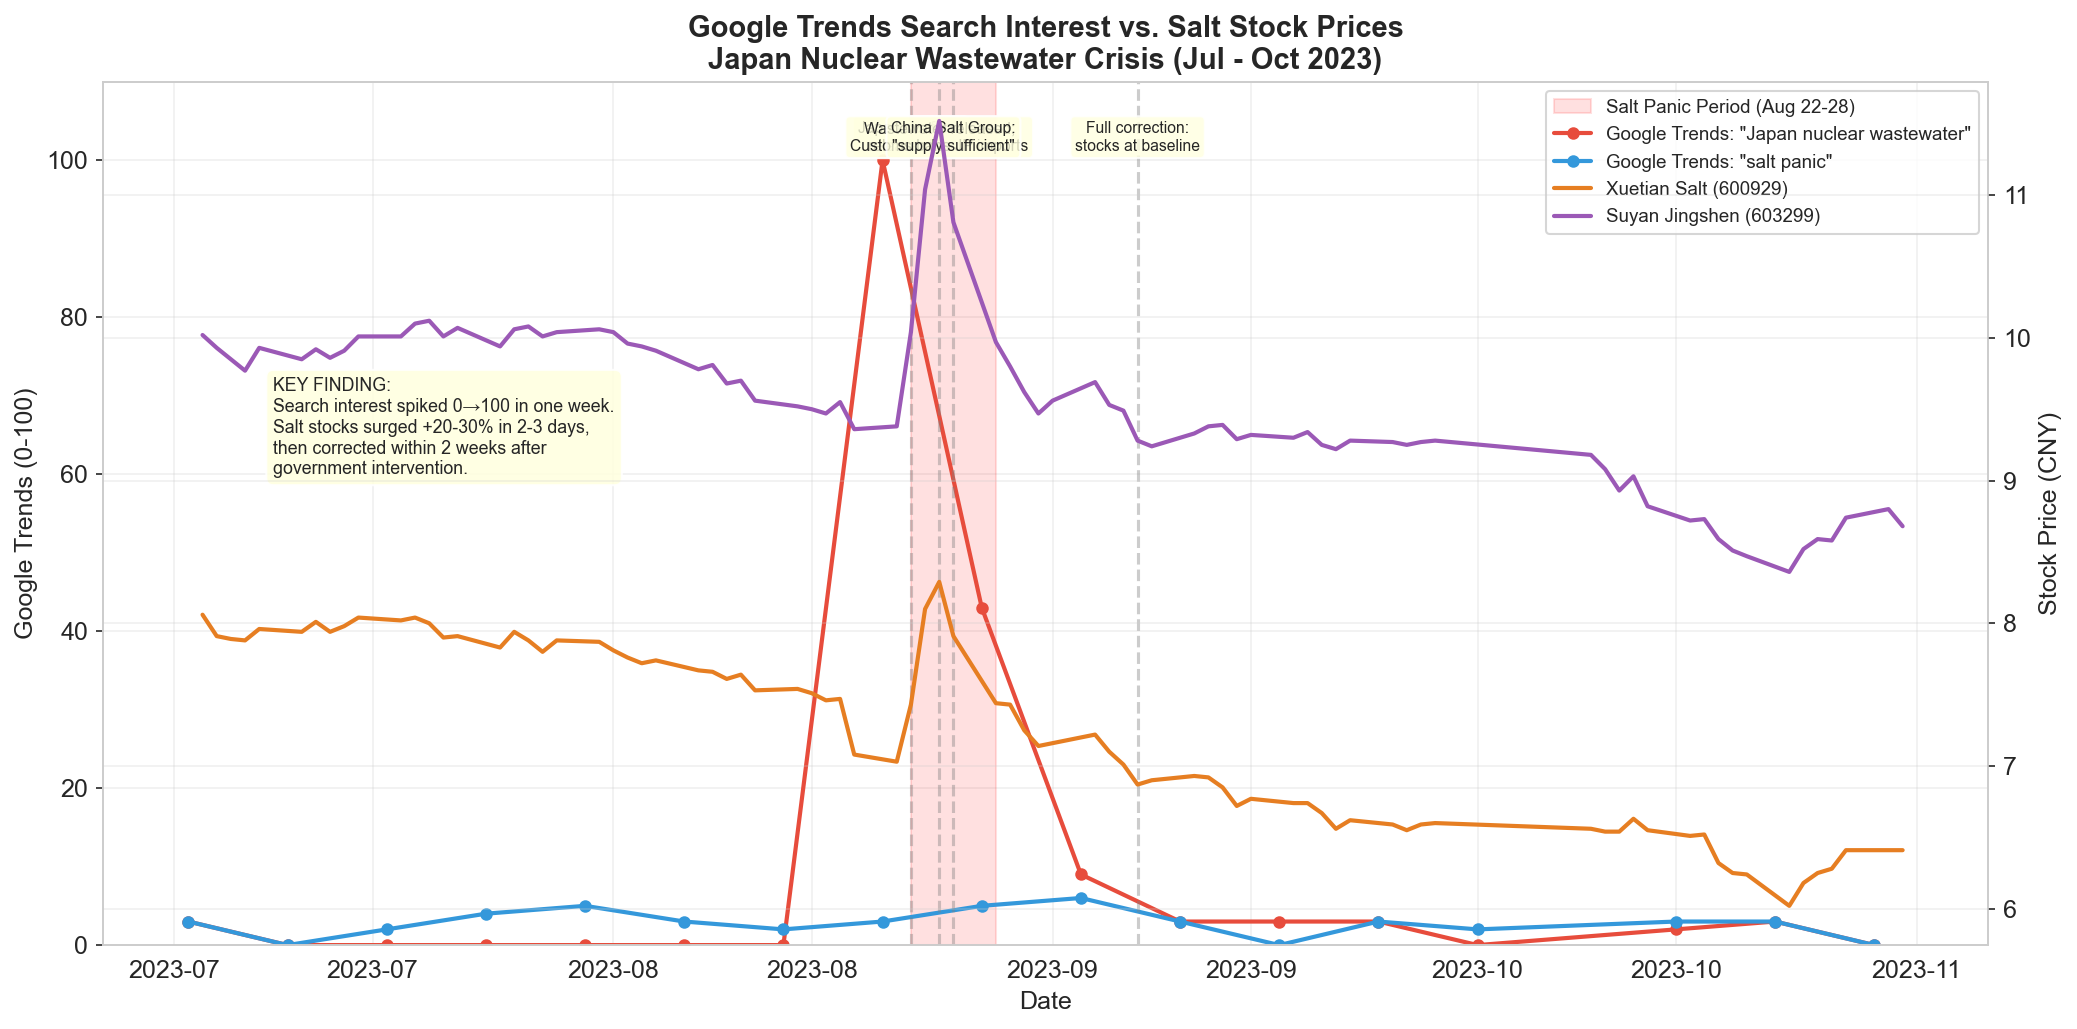
\includegraphics[width=\linewidth]{figures/Fig4_SaltPanic_Trends_vs_Stocks.png}
    \caption{Case 2: weekly salt-panic attention and salt-sector stocks. The figure shows how sharply the attention burst rises and falls, which supports the panic-coordination interpretation.}
    \label{fig:salt_trends_stocks}
\end{figure}

This case is very important, because the overflow is instantaneous. As shown in Figure~\ref{fig:salt_trends_stocks}, search attention has risen sharply, consumer panic has emerged rapidly, and the reaction of the market and the government occurs in the same narrow window. Compared with the Nongfu Spring case, the salt panic case is shorter and influences more people. It shows how online visibility coordinates behavior around a simple consumer behavior: buying and storing salt. Figure~\ref{fig:salt_price_volume} shows the peak trading volume of the sudden cycle and the subsequent rapid reversal.

\begin{figure}[t]
    \centering
    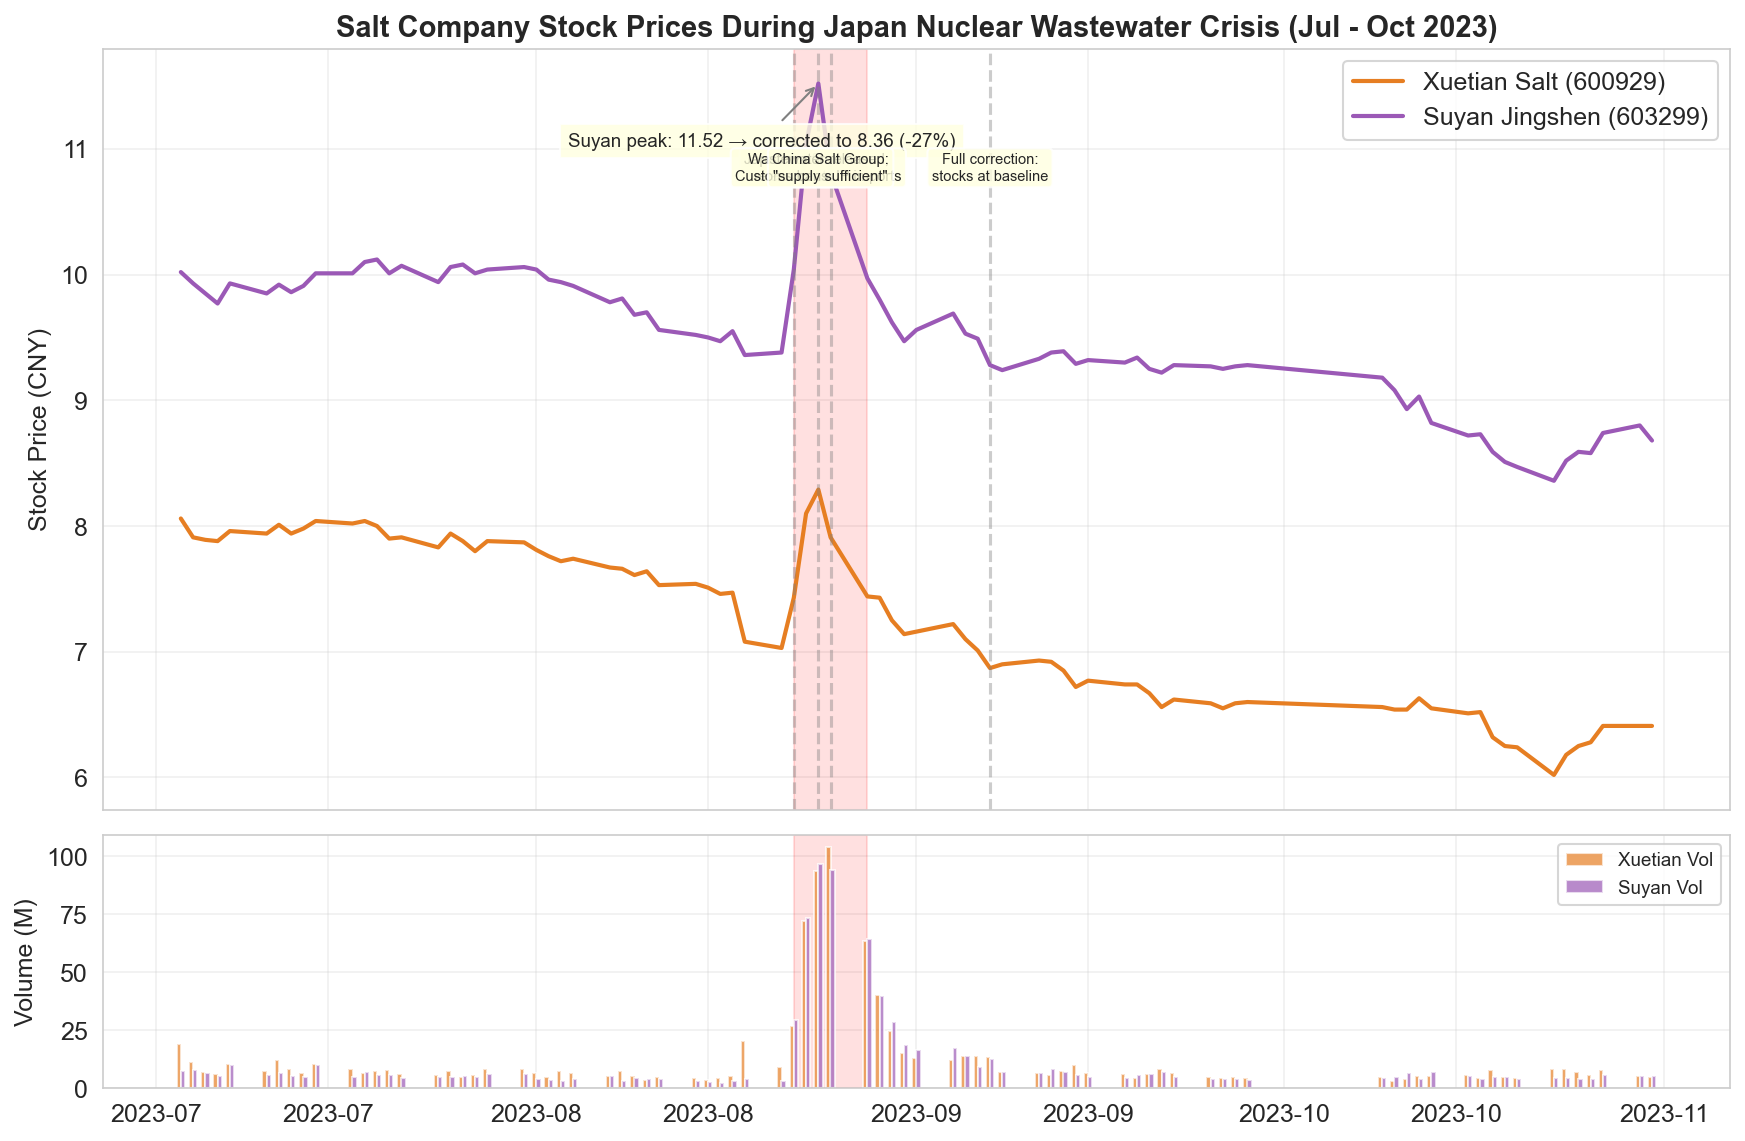
\includegraphics[width=\linewidth]{figures/Fig5_SaltPanic_Price_Volume.png}
    \caption{Case 2: salt-stock price and volume. Extraordinary burst-period volume and the quick reversal help distinguish panic coordination from the longer persistence seen in Case 1.}
    \label{fig:salt_price_volume}
\end{figure}

The market reaction is obvious in the price changes and trading volume of salt-related companies. However, the more important analysis point is not only stock fluctuations. This is a combination of consumer hoarding and government supply guarantee. The government's response shows that when online trends cause obvious market chaos or shortage expectations, the country can respond not only by adjusting discussions, but also by ensuring supply, warning of hoarding or stabilizing prices\cite{reuters2023saltmaker}.

Therefore, the salt panic supports the newspaper's statement that consumer goods spillage can be based on the market and governance. This is still not a purely causal test, because wastewater discharge itself is a major external event. But the timing shows that online visibility amplifies consumer actions and makes the problem sufficient for state intervention.
\FloatBarrier

\subsection{Case 3: Lianhua Qingwen and Medicine-Demand Repricing}
The Lianhua Qingwen case represents a medicine-demand and pharmaceutical-repricing pathway. Unlike Nongfu Spring, this was not a boycott. Unlike the salt panic, it was not a simple hoarding event around a basic commodity. The trigger was the reopening period after China began moving away from Zero COVID controls in late 2022. As infection concerns increased, public attention turned toward COVID-related medicines, including Lianhua Qingwen \cite{statecouncil2022tenmeasures,afp2022medicines}.

This case shows how online attention can shape demand expectations. The controversy around Lianhua Qingwen was connected to both public-health uncertainty and consumer search for treatment options. Product-specific attention became embedded in a broader reopening-era health-information environment, and Figure~\ref{fig:lianhua_trends_yiling} places that surge alongside Yiling Pharmaceutical's market movement. This distinction matters because the case should not be interpreted as a general pharmaceutical rally. The strongest market response was concentrated around the company most directly linked to the product \cite{duan2021covid,li2022panic,afp2022medicines}.

\begin{figure}[t]
    \centering
    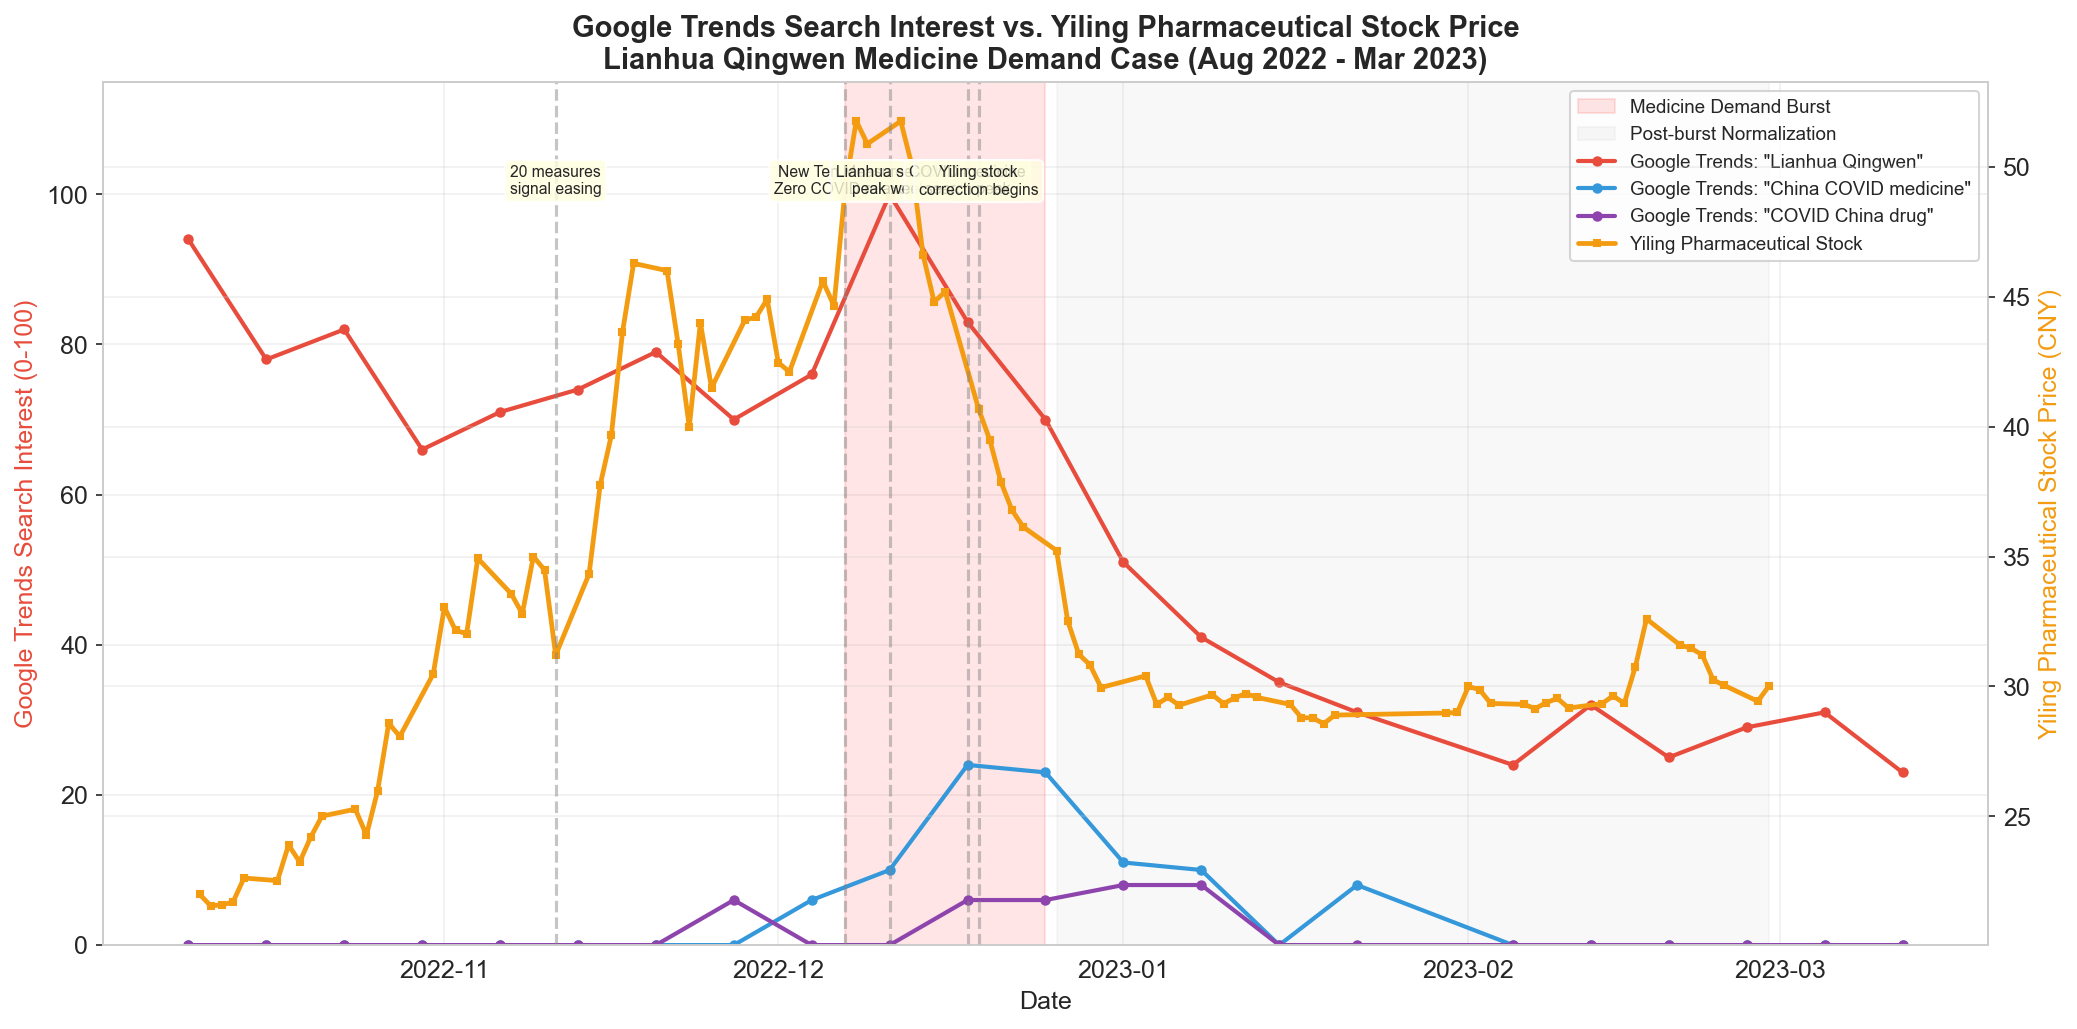
\includegraphics[width=\linewidth]{figures/C4_Fig1_Lianhua_Trends_vs_Yiling.png}
    \caption{Case 3: weekly Lianhua Qingwen attention and Yiling Pharmaceutical stock price. The figure highlights the post-reopening attention surge and its concentration around the product-linked firm.}
    \label{fig:lianhua_trends_yiling}
\end{figure}

The comparison with Tongrentang helps clarify the mechanism. If the effect were only a broad traditional-medicine or pharmaceutical-sector rally, both firms would be expected to move similarly. Instead, the product-linked firm showed a stronger rally and clearer correction. This pattern supports the interpretation that product-specific online attention and medicine-demand expectations were associated with the repricing. Figure~\ref{fig:lianhua_yiling_tongrentang} then compares the two stocks directly and shows the sharper rally-correction cycle in Yiling.

\begin{figure}[t]
    \centering
    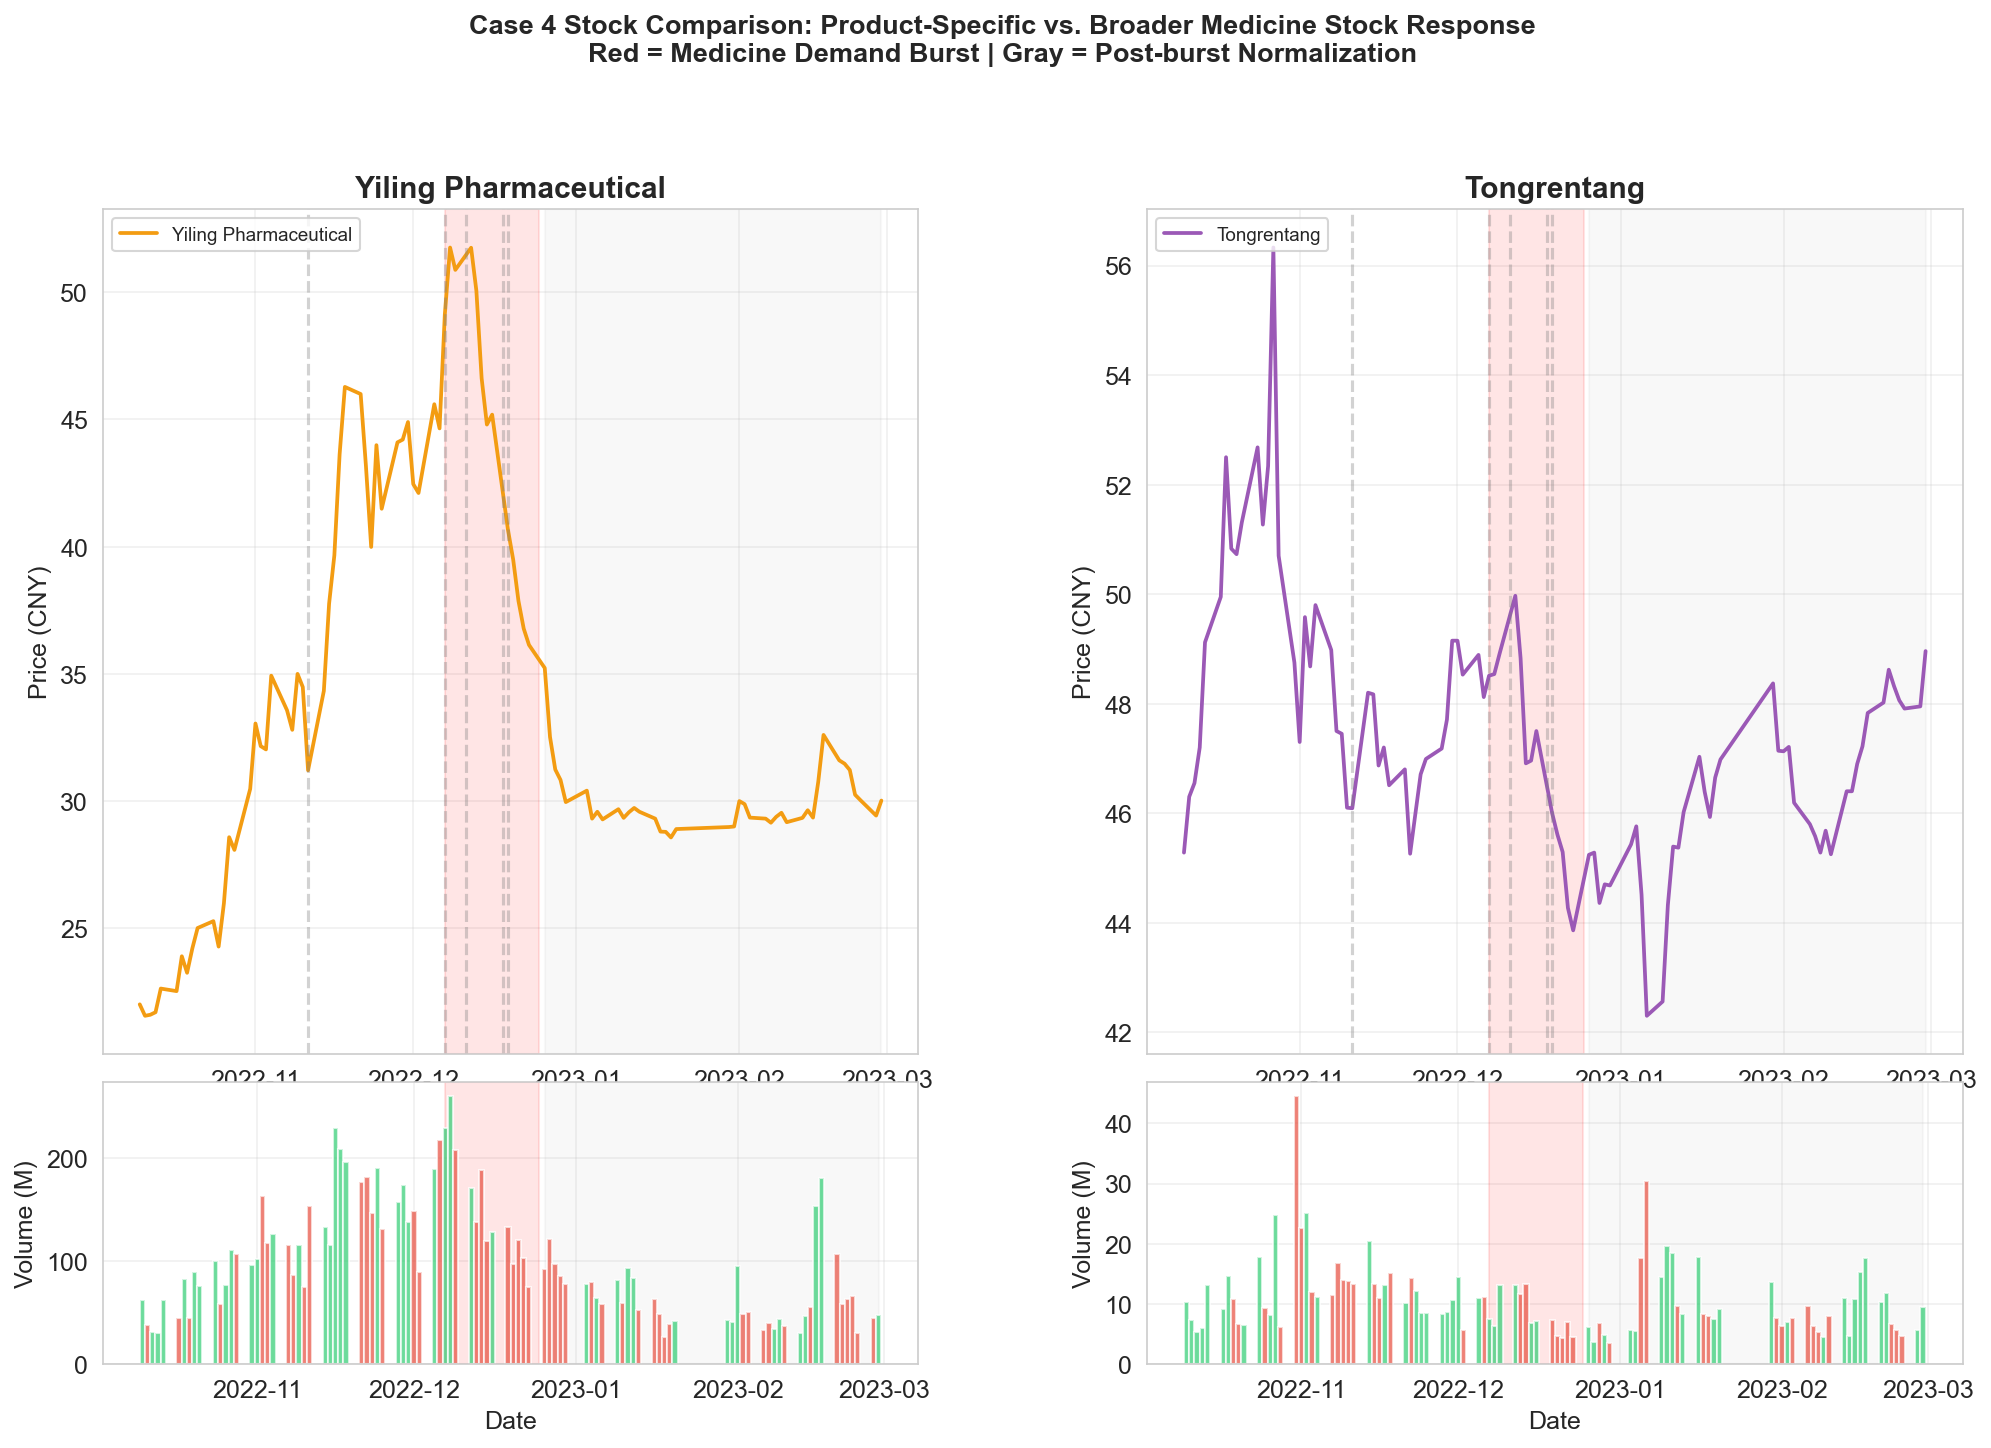
\includegraphics[width=\linewidth]{figures/C4_Fig3_Yiling_Tongrentang_Price_Volume.png}
    \caption{Case 3: Yiling Pharmaceutical versus Tongrentang. The comparison shows stronger direct exposure and a clearer correction in Yiling, which helps distinguish product-linked repricing from a broad sector rally.}
    \label{fig:lianhua_yiling_tongrentang}
\end{figure}

The Lianhua Qingwen case also shows that spillovers can reverse. Online attention may produce short-term demand expectations, but once the initial demand shock fades or expectations adjust, market correction can follow. This makes the case analytically different from Nongfu Spring's persistent reputational damage and the salt panic's short commodity shock.
\FloatBarrier

\subsection{Boundary Case: Urumqi Fire, Protest Visibility, and Government Response}
The Urumqi fire is treated as a boundary case rather than a consumer-goods case. Its inclusion is justified because it shows what happens when online attention becomes politically sensitive and difficult to contain. The trigger was the residential fire in Urumqi on November 24, 2022. Online mourning and anger became connected to broader criticism of Zero COVID controls, and the event became part of a wider protest signal \cite{dw2022urumqiprotests}. Figure~\ref{fig:urumqi_trends_airchina} situates the protest-attention spike alongside Air China's reopening-sensitive price movement.

\begin{figure}[t]
    \centering
    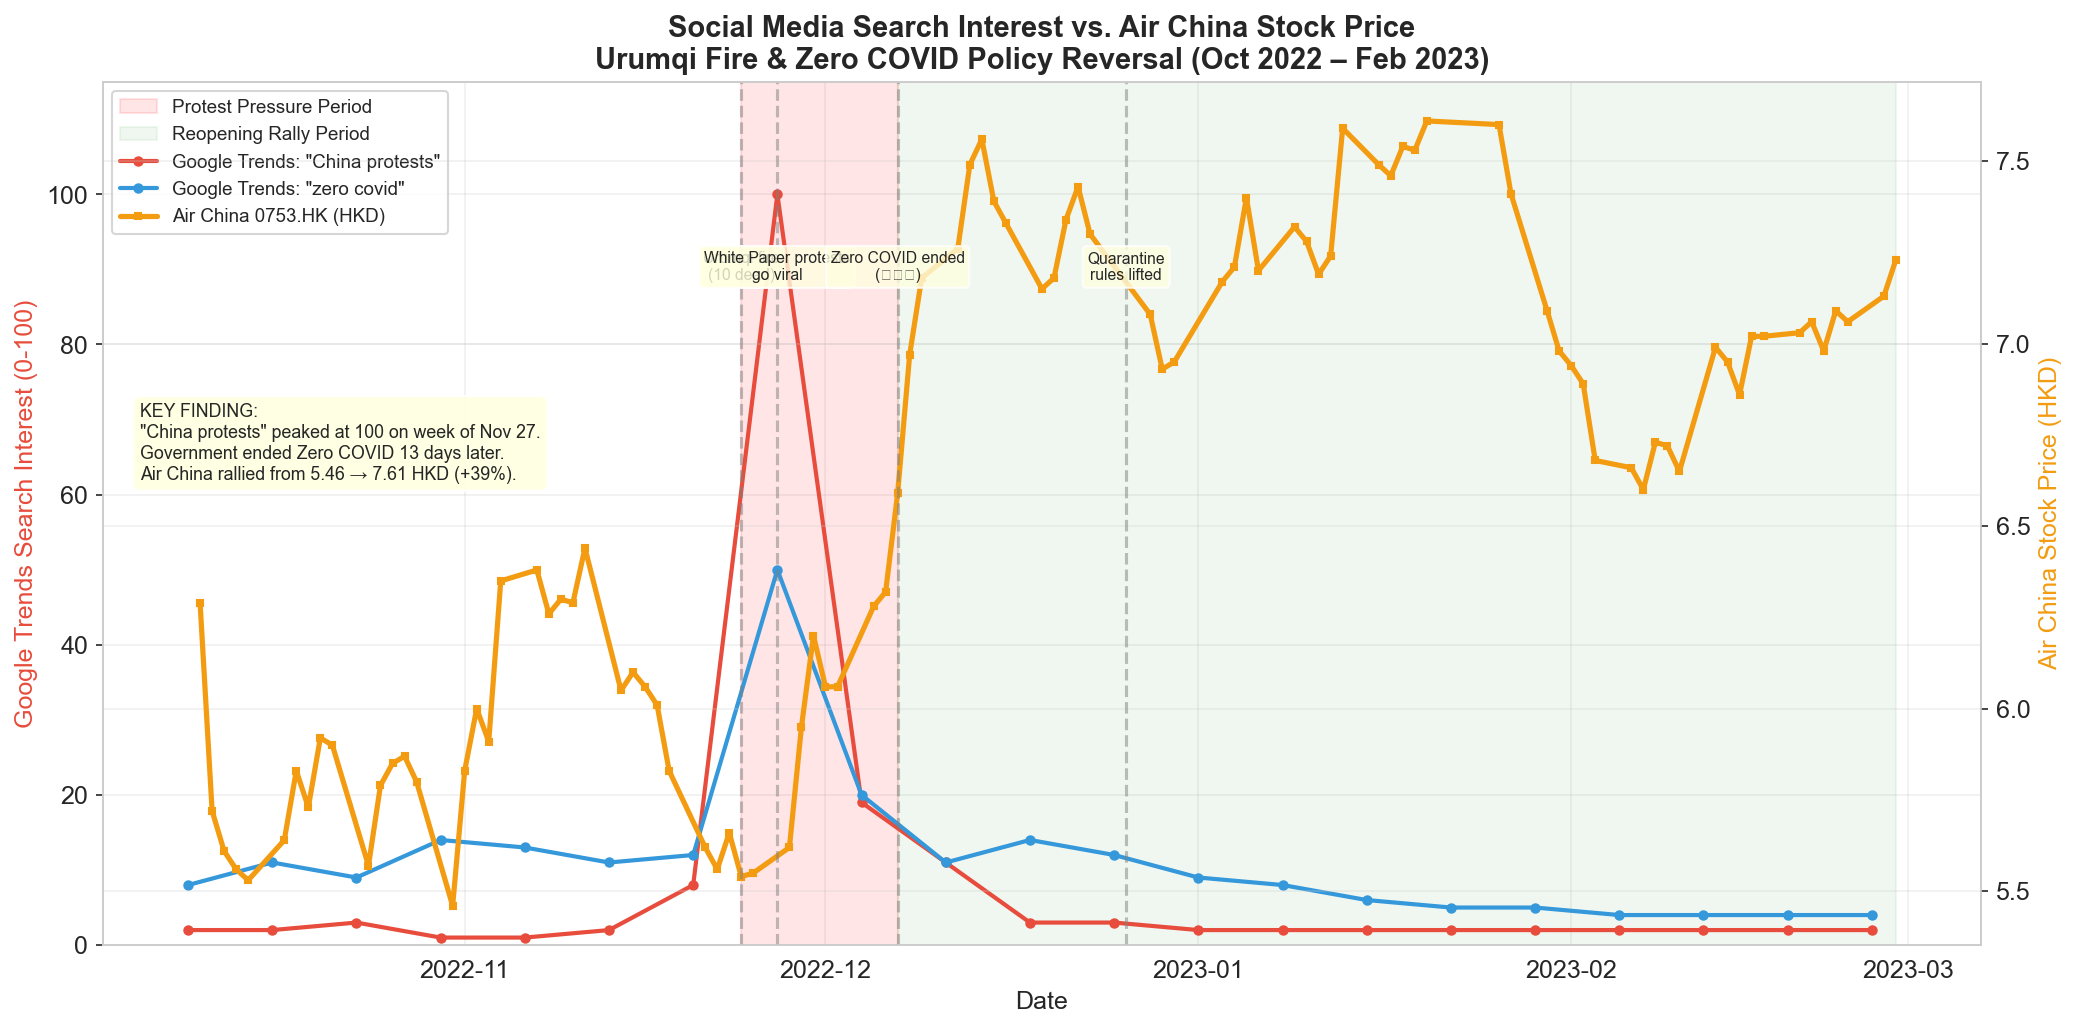
\includegraphics[width=\linewidth]{figures/C3_Fig1_Urumqi_Trends_vs_AirChina.png}
    \caption{Boundary case: protest-related search attention and Air China stock price. The figure compresses visibility, policy reversal, and reopening-sensitive repricing into one short window.}
    \label{fig:urumqi_trends_airchina}
\end{figure}

The main spillover in this case was not consumer purchasing behavior. It was policy pressure. Figure~\ref{fig:urumqi_trends_airchina} situates the protest-related attention window alongside reopening-sensitive market movement. The case therefore marks the outer boundary of the paper's argument: when online attention becomes sufficiently visible, platform control may shape the pathway of visibility, but it may not fully prevent the issue from becoming legible to the government.

The event sequence suggests a compressed relationship between protest visibility, policy change, and market repricing. Reopening-sensitive stocks began to move around the protest and policy-reversal window, while the December 7 ``New Ten Measures'' marked a major change in China's Zero COVID policy \cite{statecouncil2022tenmeasures,dw2022easing}. This does not mean that online attention alone caused the policy shift. The policy environment was already under pressure from economic, epidemiological, and administrative factors. However, the case shows how a politically sensitive attention event can become associated with state response once it reaches sufficient visibility \cite{zheng2021responsiveness,ruan2021punishment}. Figure~\ref{fig:urumqi_haidilao_tripcom} then shows that the repricing extended beyond Air China to Haidilao and Trip.com.

\begin{figure}[t]
    \centering
    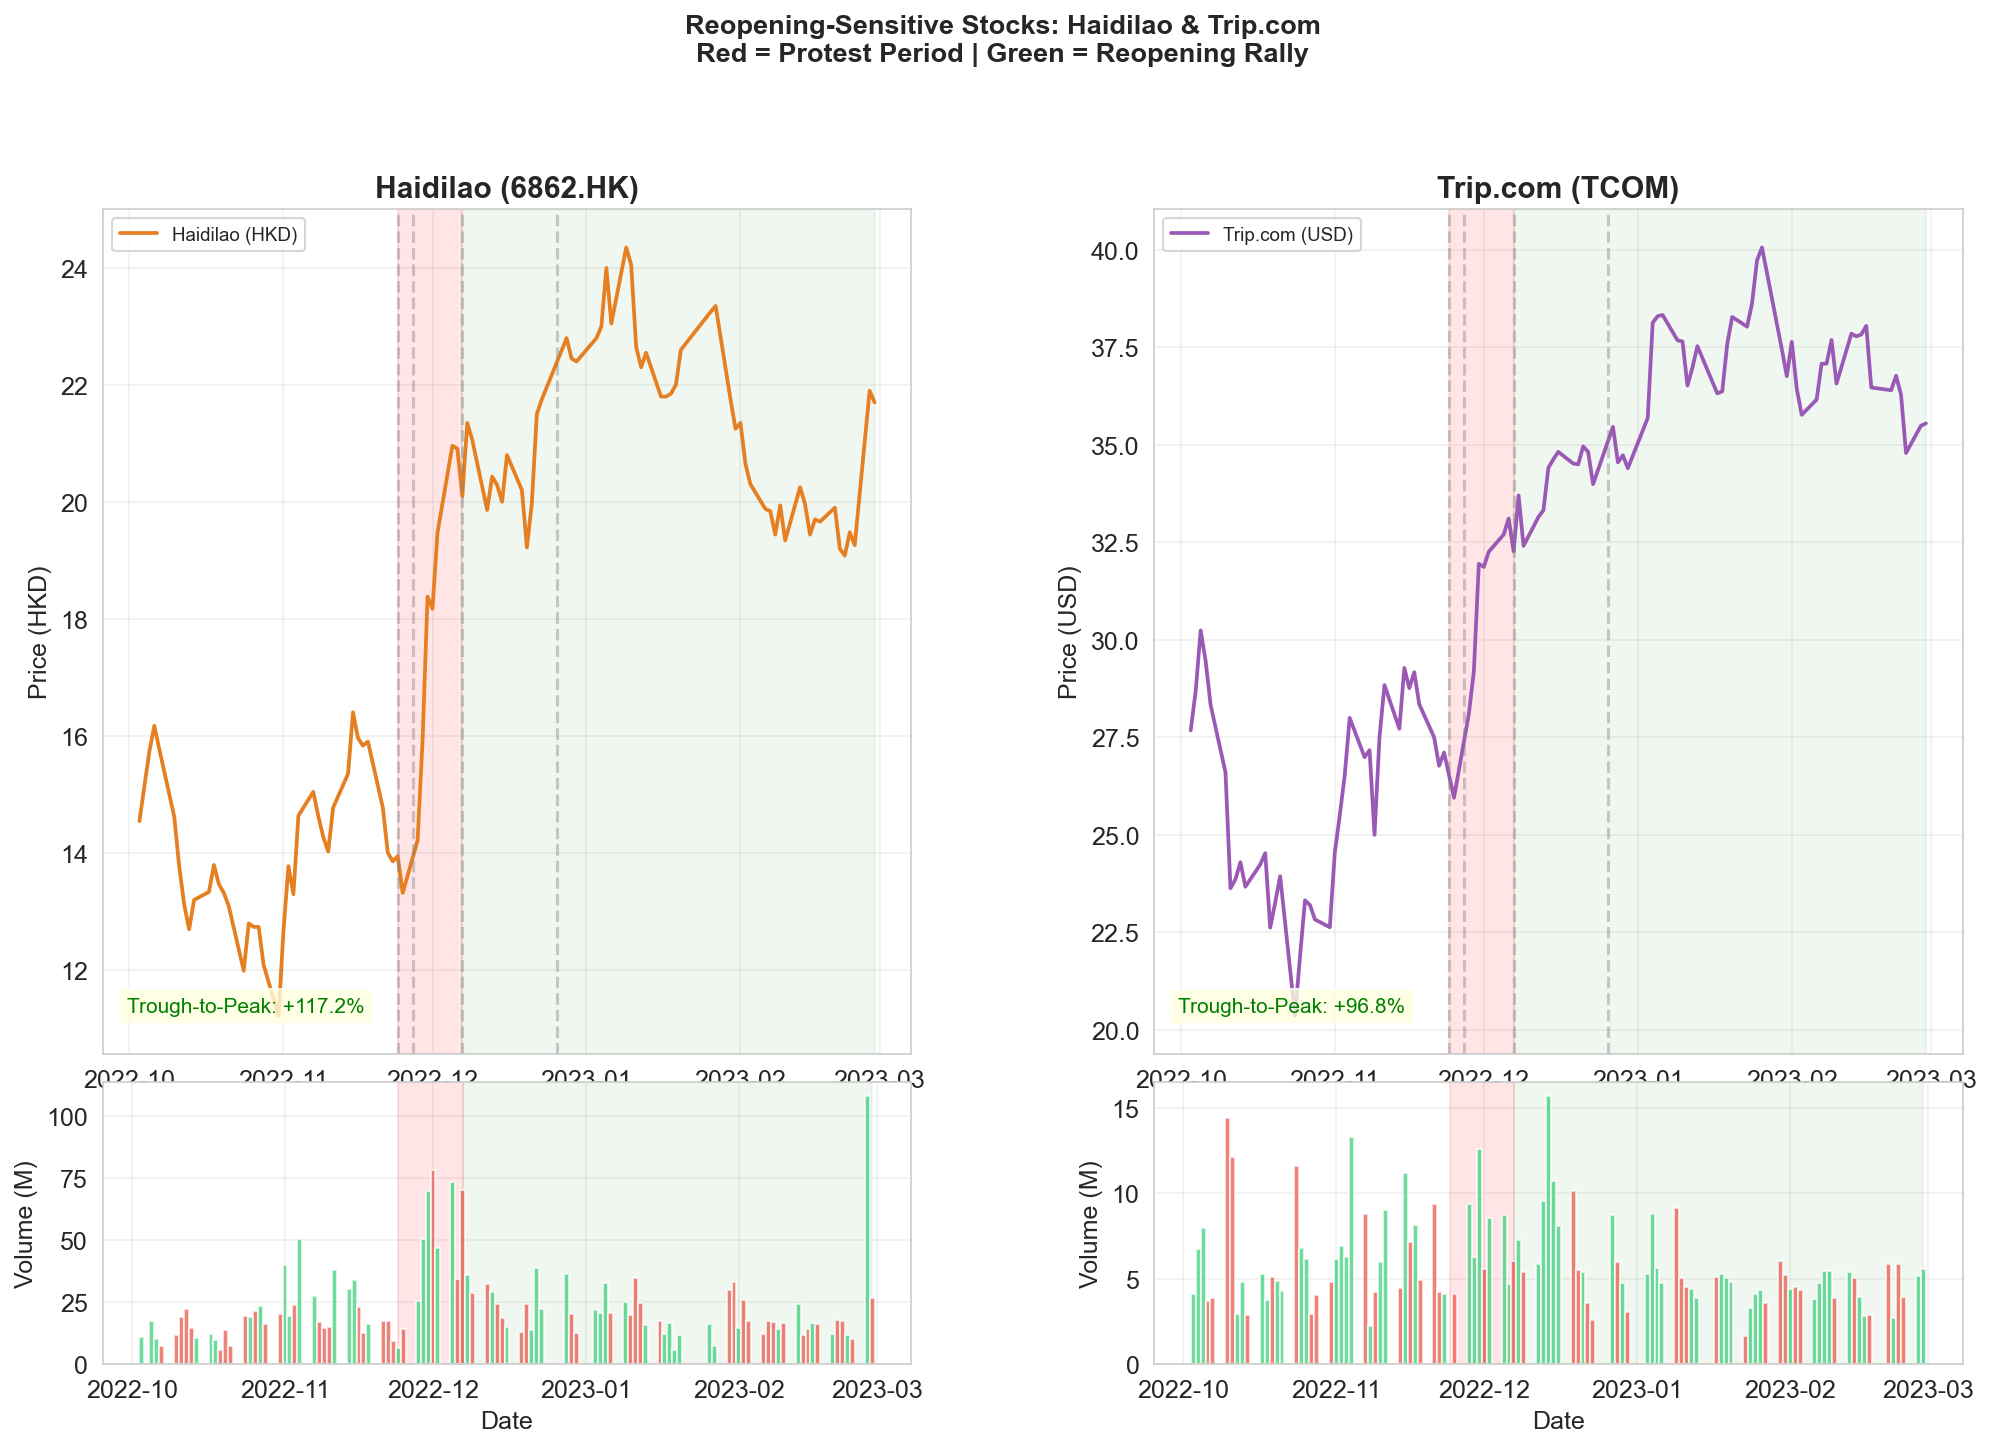
\includegraphics[width=\linewidth]{figures/C3_Fig3_Haidilao_TripCom_Price_Volume.png}
    \caption{Boundary case: Haidilao and Trip.com during the protest and reopening windows. The comparison shows that repricing spread across reopening-sensitive firms rather than staying confined to one stock.}
    \label{fig:urumqi_haidilao_tripcom}
\end{figure}

As a boundary case, Urumqi helps clarify the difference between consumer-goods spillover and policy spillover. In the first three cases, online visibility is associated mainly with consumer behavior, brand perception, or market expectations. In the Urumqi case, visibility is associated with governance response. The case therefore supports the broader framework while remaining analytically distinct from the consumer-goods cases.

\subsection{Cross-Case Comparison}
The four cases show that visibility breakthroughs do not produce one uniform type of offline effect. Instead, the spillover depends on the event type.

Nongfu Spring shows a brand-boycott pathway. The controversy developed through reputational conflict and produced a longer-lasting market decline. Salt panic shows a panic-buying pathway. The trigger was sudden, the attention spike was intense, and the response included both consumer hoarding and official supply reassurance. Lianhua Qingwen shows a medicine-demand pathway. The attention burst was connected to reopening-era health uncertainty, producing product-linked repricing followed by correction. Urumqi shows a boundary policy pathway. The attention was politically sensitive, and the main spillover was government response rather than consumer behavior.

\begin{table*}[!b]
\centering
\caption{Cross-Case Comparison}
\label{tab:cross_case}
{\footnotesize
\setlength{\tabcolsep}{4pt}
\begin{tabular}{p{0.13\textwidth}p{0.15\textwidth}p{0.16\textwidth}p{0.15\textwidth}p{0.10\textwidth}p{0.17\textwidth}}
\toprule
Case & Trigger & Pathway & Spillover & Duration & Main inference \\
\midrule
Nongfu Spring & Brand controversy & Brand boycott & Reputation and stock decline & Persistent & Longer market reassessment \\
Salt panic & Wastewater release & Panic buying & Hoarding, volatility, reassurance & Short and intense & Immediate market and governance response \\
Lianhua Qingwen & Medicine concern & Product demand & Repricing and correction & Burst/correction & Product-linked demand expectations \\
Urumqi fire & Fire and protest visibility & Boundary policy pathway & Government response and reopening repricing & Compressed & Policy response, not consumer-goods spillover \\
\bottomrule
\end{tabular}
}
\end{table*}

This comparison supports the paper's main claim. Online controversies in China become consequential not simply because they are discussed online, but because they move beyond their original platform spaces and become visible to actors outside the platform: consumers, investors, firms, regulators, or state agencies. The same visibility breakthrough can produce different outcomes depending on whether the issue concerns a brand, a basic commodity, a health product, or a politically sensitive event.

At the same time, the comparison also limits the paper's claims. The cases are not representative of all online controversies in China. They are most-likely cases selected because each has a visible trigger and observable spillover. The findings should therefore be read as a theory-building comparison rather than as a population-level test.

\section{Discussion}
The paper's main finding is that online attention becomes consequential through visibility breakthrough, not through platform discussion alone. In China's governed platform environment, visibility is shaped by both amplification and restriction. Algorithms, trending lists, influencer participation, reposting, and short-video circulation can increase visibility, while moderation, censorship, search filtering, and platform intervention can reduce or redirect it. The survey results suggest that respondents perceive both processes at the same time: Chinese platform control is not viewed as simply suppressive, but as a system that can both amplify and constrain public attention.

This helps explain why the paper uses a threshold framework. A controversy may exist online without producing obvious offline consequences. But when it becomes visible enough to move across platforms and into broader public attention, it can become legible to consumers, investors, firms, and government actors. In the cases examined here, that visibility breakthrough is associated with different forms of spillover: brand damage, panic buying, medicine-demand repricing, and policy response.

The Google Trends limitation is central to this interpretation. Since Google Trends cannot directly measure domestic Chinese social-media discussion, it should not be overread. Its value is narrower: it helps identify moments when China-related controversies became visible in a broader search and public-attention environment. The survey evidence partially strengthens this interpretation by showing that the selected events were widely recognized among respondents with Chinese social-media experience and that many respondents perceived both consumer and government effects from large online trends.

The boundary case also matters. The Urumqi fire shows that platform control does not mean full control over public attention. Under certain conditions, politically sensitive attention may become visible enough that policy response becomes more likely. This does not prove that online attention caused the Zero COVID reversal, but it shows that major online visibility can become part of a broader pressure environment.

\section{Limitations}
This paper has several limitations.

First, the case selection is based on purposive but not representative. Selecting those four cases because they have recently happened, have high visibility, and have data accessibility. Therefore, they should not be seen as a random sample of Chinese online controversies.

Second, we do not have the right to access the historical platform data directly from Weibo, Douyin, WeChat, or Xiaohongshu. So this causes the analysis to be unable to measure the total domestic discussion volume, sentiment structure, moderation process, or algorithmic pathway of each event.

Third, Google Trends is not a perfect substitution. Although it is useful for observing broader cross-platform public-salience trends, it cannot directly reflect Chinese domestic social media attention. The paper, therefore, uses Google Trends only as one of several signals.

Fourth, the survey cannot be regarded as representative of the nation. The people surveyed are mainly students, young workers, Chinese immigrants, and international students who use Chinese social media and are familiar with U.S. or Western social media. So, the survey is useful for perception-based triangulation but not for estimating overall Chinese public opinion.

Fifth, the paper cannot establish causality. This is because market movements, consumer behavior, and government responses are usually affected by broader news shocks, firm fundamentals, policy changes, economic conditions, and public health developments. As a result, the paper uses careful wording such as ``associated with,'' ``temporally aligned with,'' and ``suggests'' rather than claiming direct causal effects.

\section{Conclusion}
This paper examined how social-media-originated controversies in China move beyond platform-specific discussion and become associated with offline spillovers. Its central argument is that online trends become consequential when they break through a governed visibility environment and enter broader public attention. Once this happens, the spillover pathway depends on the type of event.

The three consumer-goods cases show different mechanisms. Nongfu Spring illustrates how online brand controversy can become associated with reputational damage and market decline. The salt panic shows how public-health fear can become associated with panic buying, commodity-stock volatility, and government supply reassurance. Lianhua Qingwen shows how reopening-era health uncertainty can become associated with product-specific medicine demand and pharmaceutical repricing. The Urumqi fire, treated as a boundary case, shows how politically sensitive attention can become associated with government response and policy change.

The paper does not claim that Google Trends directly measures Chinese social-media attention. Nor does it claim that online attention alone caused the observed market or policy outcomes. Instead, it uses Google Trends as a secondary indicator of broader public salience and triangulates it with survey responses, event timelines, market indicators, media reports, and policy actions. This approach is limited, but it gives a more careful way to study online spillover when direct platform data are unavailable.

The broader implication is that platform control does not eliminate online spillover. It changes the conditions under which spillover occurs. In China, some online controversies may remain contained, fragmented, or short-lived. Others break through the visibility threshold and become meaningful to consumers, firms, investors, or the government. Understanding that threshold is essential for explaining when online attention becomes more than online attention.

\bibliographystyle{IEEEtran}
\bibliography{references}

\clearpage
\appendices
\setcounter{figure}{0}
\renewcommand{\thefigure}{A\arabic{figure}}
\section{Supplementary Figures}
Figure~\ref{fig:appendix_survey} retains one cleaned survey summary visualization from \texttt{survey\_outputs/}.

\begin{figure}[H]
    \centering
    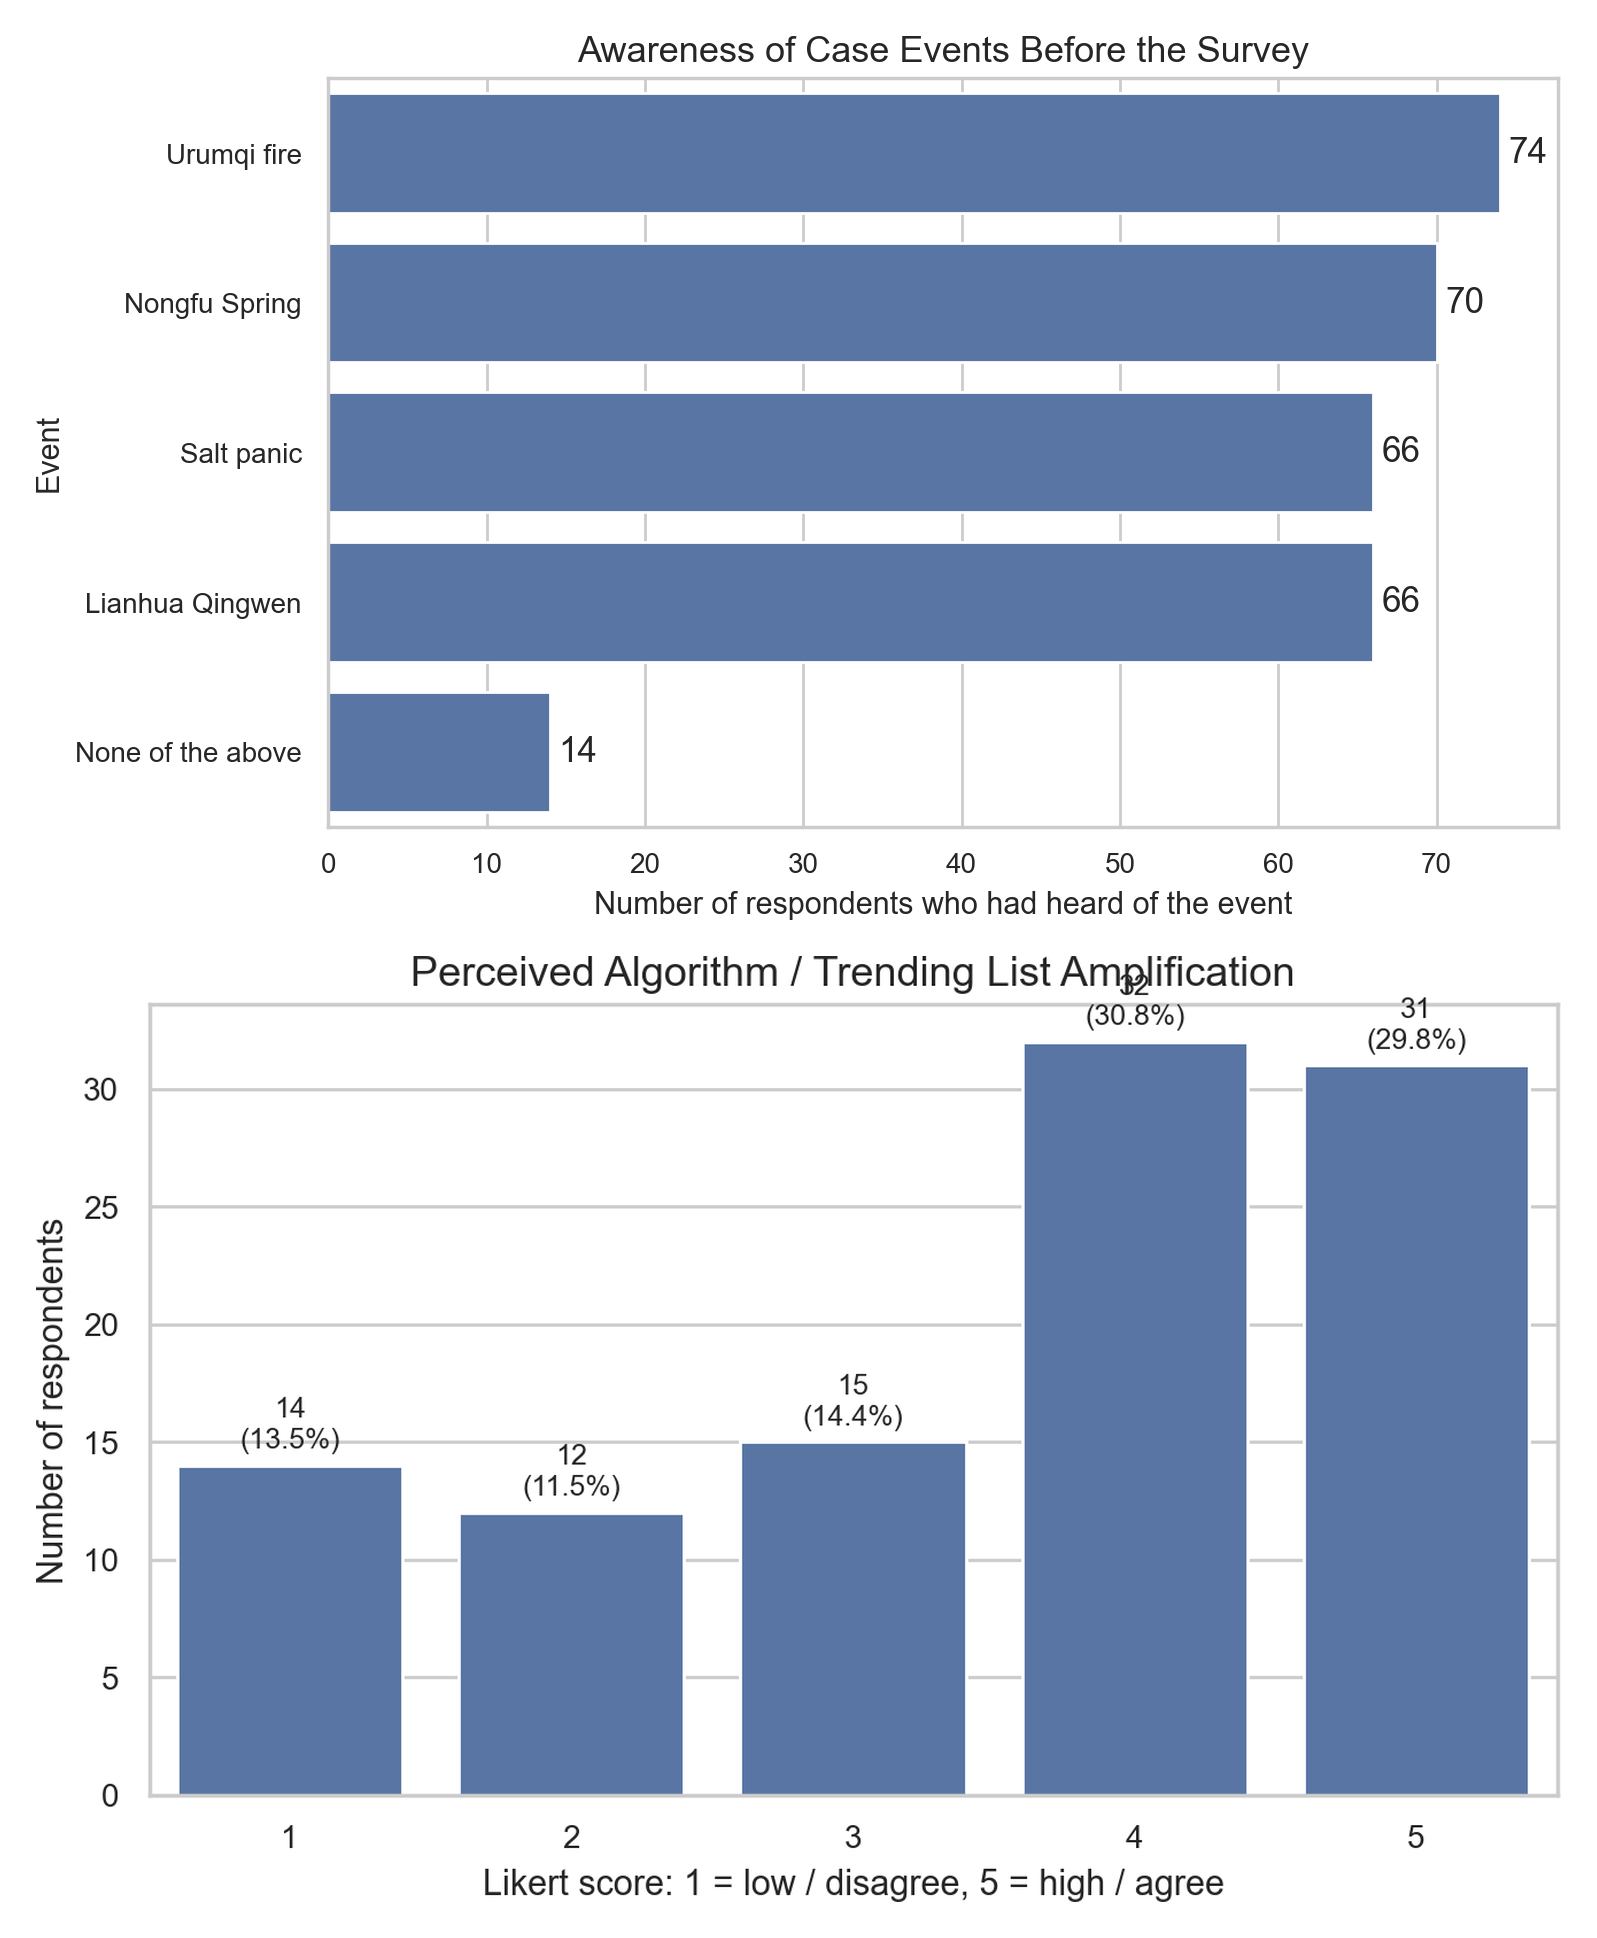
\includegraphics[width=\linewidth]{../survey_outputs/clean_survey_summary.png}
    \caption{Survey-based triangulation of event awareness and perceived platform control. Data: author survey, $n=104$.}
    \label{fig:appendix_survey}
\end{figure}

\end{document}
